%%%%HEADER
\documentclass[twocolumn]{article}
\usepackage[a4paper, margin=0.7in, columnsep=30pt]{geometry}
\usepackage{amsmath, amssymb, graphicx, hyperref}
\usepackage[most,skins,breakable]{tcolorbox}
\usepackage[symbol]{footmisc}
\usetikzlibrary{calc}
\usepackage{xcolor}
\usepackage{caption}
\usepackage{transparent}
% \usepackage{algorithm}
% \usepackage{algpseudocodex}
\usepackage{tikz}
\usepackage{listings}
\usepackage{changepage}   % for the adjustwidth environment
\usetikzlibrary{arrows.meta, positioning}
\tcbuselibrary{listingsutf8}
\usepackage{microtype}
\usepackage{blindtext}
\usepackage{bookmark}
\usepackage{breqn}
\usepackage[backend=biber,style=numeric]{biblatex} % 
\addbibresource{../references.bib}

% Define style for the listings environment
\lstdefinestyle{mystyle}{
    basicstyle=\ttfamily\small,
    breaklines=true,
    escapeinside={(*@}{@*)}, % Allows math mode within listings
    numbers=left,
    numberstyle=\tiny,
    frame=single,
    keywordstyle=\color{blue}\bfseries,
    commentstyle=\color{green!50!black},
    stringstyle=\color{red}
}


\def\reals{\mathbb{R}}
% Define the custom definition box and command
\newtcolorbox{mydefinition}[2][]{%
    text width=0.95\columnwidth,
    before=\vspace{1mm}, 
    after=\vspace{1mm}, 
    colback=gray!5, % Background color (light gray)
    colframe=black!70,  % Border color
    coltitle=gray!10,  % Title color
    fonttitle=\bfseries, % Title font style
    sharp corners,   % Box style
    left=2pt,
    breakable,
    right=2pt,
    top=2pt,
    bottom=2pt,
    enhanced jigsaw,
    title=Definition: {#1},         % Title passed as the first argument
    colupper=black,  % Ensure proper content handling
    pad at break*=1pc,
    overlay first and middle={
        \coordinate (A1) at ($(interior.south east) + (-10pt,5pt)$);
        \coordinate (C1) at ($(interior.south east) + (-6pt,7.5pt)$);
        \draw[fill=black!50] (A1) -- +(0,5pt) -- (C1) -- cycle;
    }
    }
    
\newcommand{\definition}[2]{%
    \noindent%
    \begin{mydefinition}[#1]%
        .#2%
    \end{mydefinition}%
    \noindent
}

\newtcolorbox{myexample}[2][]{%
    text width=0.95\columnwidth,
    before=\vspace{1mm}, 
    after=\vspace{1mm}, 
    colback=orange!2, % Background color (light orange)
    colframe=black!70,  % Border color
    coltitle=gray!10,  % Title color
    fonttitle=\bfseries, % Title font style
    sharp corners,   % Box style
    left=2pt,
    right=2pt,
    top=2pt,
    bottom=2pt,
    breakable,
    title=Intuition: {#1},         % Title passed as the first argument
    pad at break*=1pc,
    overlay first and middle={
        \coordinate (A1) at ($(interior.south east) + (-10pt,5pt)$);
        \coordinate (C1) at ($(interior.south east) + (-6pt,7.5pt)$);
        \draw[fill=black!50] (A1) -- +(0,5pt) -- (C1) -- cycle;
    }
}

\newcommand{\example}[2]{%
    \noindent%
    \begin{myexample}[#1]%
    .#2%
    \end{myexample}%
    \noindent
}

\newtcolorbox{algobox}[2][]{%
    text width=0.95\columnwidth,
    before=\vspace{1mm}, 
    after=\vspace{1mm}, 
    colback=blue!5, % Background color (light gray)
    colframe=black!70,  % Border color
    coltitle=gray!10,  % Title color
    fonttitle=\bfseries, % Title font style
    sharp corners,   % Box style
    left=2pt,
    right=2pt,
    top=2pt,
    bottom=2pt,
    breakable,
    title=Algorithm: {#1},         % Title passed as the first argument
    pad at break*=1pc,
    overlay first and middle={
        \coordinate (A1) at ($(interior.south east) + (-10pt,5pt)$);
        \coordinate (C1) at ($(interior.south east) + (-6pt,7.5pt)$);
        \draw[fill=black!50] (A1) -- +(0,5pt) -- (C1) -- cycle;
    }
}

\newcommand{\algorithmbox}[2]{%
\noindent%
    \begin{algobox}[#1]%
    .#2%
    \end{algobox}%
    \noindent
}


\newtcolorbox{questionbox}[2][]{%
    text width=0.95\columnwidth,
    before=\vspace{1mm}, 
    after=\vspace{1mm}, 
    colback=orange!3, % Background color (light orange)
    colframe=black!70,  % Border color
    coltitle=gray!10,  % Title color
    fonttitle=\bfseries, % Title font style
    sharp corners,   % Box style
    left=2pt,
    right=2pt,
    top=2pt,
    bottom=2pt,
    breakable,
    title=Question: {#1},         % Title passed as the first argument
    pad at break*=1pc,
    overlay first and middle={
        \coordinate (A1) at ($(interior.south east) + (-10pt,5pt)$);
        \coordinate (C1) at ($(interior.south east) + (-6pt,7.5pt)$);
        \draw[fill=black!50] (A1) -- +(0,5pt) -- (C1) -- cycle;
    }
}

\newcommand{\question}[2]{%
\noindent%
    \begin{questionbox}[#1]%
    .#2%
    \end{questionbox}%
    \noindent
}

%%%HEADER

\def\COMPILINGFROMMAIN{}
\begin{document}

\title{Two-Column Layout Example}
\author{Theo Computer Scientist}
\date{\today}
\maketitle


\begin{abstract}
In this thesis we discuss details of implementing a probabilistic numerical solver for partial differential equations whose spatial domain is not a vector space. We cover topics including the concept of the metric tensor, embeddings of manifolds, mesh representations and refinement, discrete differential operators, ODEs, PDEs, and SDEs, numerical linear algebra, state space models, the (extended) Kálmán-filter and -smoother, and numerical stability. We conclude with experiments that test the efficiency of physically informed prior solutions in non-euclidean domains.

We have structured the thesis as a guide on how to implement and follow the results, and we try to motivate the steps to the best of our efforts.
\end{abstract}

\ref{sec:manifolds}
\ref{sec:pde}
\ref{sec:prior}
\ref{sec:residual}
\ref{sec:matrix_exponential}
\ref{sec:kalman_filter}

\section{Overview}\label{sec:overview}
\ifdefined\COMPILINGFROMMAIN
\else
    %%%%HEADER
\documentclass[twocolumn]{article}
\usepackage[a4paper, margin=0.7in, columnsep=30pt]{geometry}
\usepackage{amsmath, amssymb, graphicx, hyperref}
\usepackage[most,skins,breakable]{tcolorbox}
\usepackage[symbol]{footmisc}
\usetikzlibrary{calc}
\usepackage{xcolor}
\usepackage{caption}
\usepackage{transparent}
% \usepackage{algorithm}
% \usepackage{algpseudocodex}
\usepackage{tikz}
\usepackage{listings}
\usepackage{changepage}   % for the adjustwidth environment
\usetikzlibrary{arrows.meta, positioning}
\tcbuselibrary{listingsutf8}
\usepackage{microtype}
\usepackage{blindtext}
\usepackage{bookmark}
\usepackage{breqn}
\usepackage[backend=biber,style=numeric]{biblatex} % 
\addbibresource{../references.bib}

% Define style for the listings environment
\lstdefinestyle{mystyle}{
    basicstyle=\ttfamily\small,
    breaklines=true,
    escapeinside={(*@}{@*)}, % Allows math mode within listings
    numbers=left,
    numberstyle=\tiny,
    frame=single,
    keywordstyle=\color{blue}\bfseries,
    commentstyle=\color{green!50!black},
    stringstyle=\color{red}
}


\def\reals{\mathbb{R}}
% Define the custom definition box and command
\newtcolorbox{mydefinition}[2][]{%
    text width=0.95\columnwidth,
    before=\vspace{1mm}, 
    after=\vspace{1mm}, 
    colback=gray!5, % Background color (light gray)
    colframe=black!70,  % Border color
    coltitle=gray!10,  % Title color
    fonttitle=\bfseries, % Title font style
    sharp corners,   % Box style
    left=2pt,
    breakable,
    right=2pt,
    top=2pt,
    bottom=2pt,
    enhanced jigsaw,
    title=Definition: {#1},         % Title passed as the first argument
    colupper=black,  % Ensure proper content handling
    pad at break*=1pc,
    overlay first and middle={
        \coordinate (A1) at ($(interior.south east) + (-10pt,5pt)$);
        \coordinate (C1) at ($(interior.south east) + (-6pt,7.5pt)$);
        \draw[fill=black!50] (A1) -- +(0,5pt) -- (C1) -- cycle;
    }
    }
    
\newcommand{\definition}[2]{%
    \noindent%
    \begin{mydefinition}[#1]%
        .#2%
    \end{mydefinition}%
    \noindent
}

\newtcolorbox{myexample}[2][]{%
    text width=0.95\columnwidth,
    before=\vspace{1mm}, 
    after=\vspace{1mm}, 
    colback=orange!2, % Background color (light orange)
    colframe=black!70,  % Border color
    coltitle=gray!10,  % Title color
    fonttitle=\bfseries, % Title font style
    sharp corners,   % Box style
    left=2pt,
    right=2pt,
    top=2pt,
    bottom=2pt,
    breakable,
    title=Intuition: {#1},         % Title passed as the first argument
    pad at break*=1pc,
    overlay first and middle={
        \coordinate (A1) at ($(interior.south east) + (-10pt,5pt)$);
        \coordinate (C1) at ($(interior.south east) + (-6pt,7.5pt)$);
        \draw[fill=black!50] (A1) -- +(0,5pt) -- (C1) -- cycle;
    }
}

\newcommand{\example}[2]{%
    \noindent%
    \begin{myexample}[#1]%
    .#2%
    \end{myexample}%
    \noindent
}

\newtcolorbox{algobox}[2][]{%
    text width=0.95\columnwidth,
    before=\vspace{1mm}, 
    after=\vspace{1mm}, 
    colback=blue!5, % Background color (light gray)
    colframe=black!70,  % Border color
    coltitle=gray!10,  % Title color
    fonttitle=\bfseries, % Title font style
    sharp corners,   % Box style
    left=2pt,
    right=2pt,
    top=2pt,
    bottom=2pt,
    breakable,
    title=Algorithm: {#1},         % Title passed as the first argument
    pad at break*=1pc,
    overlay first and middle={
        \coordinate (A1) at ($(interior.south east) + (-10pt,5pt)$);
        \coordinate (C1) at ($(interior.south east) + (-6pt,7.5pt)$);
        \draw[fill=black!50] (A1) -- +(0,5pt) -- (C1) -- cycle;
    }
}

\newcommand{\algorithmbox}[2]{%
\noindent%
    \begin{algobox}[#1]%
    .#2%
    \end{algobox}%
    \noindent
}


\newtcolorbox{questionbox}[2][]{%
    text width=0.95\columnwidth,
    before=\vspace{1mm}, 
    after=\vspace{1mm}, 
    colback=orange!3, % Background color (light orange)
    colframe=black!70,  % Border color
    coltitle=gray!10,  % Title color
    fonttitle=\bfseries, % Title font style
    sharp corners,   % Box style
    left=2pt,
    right=2pt,
    top=2pt,
    bottom=2pt,
    breakable,
    title=Question: {#1},         % Title passed as the first argument
    pad at break*=1pc,
    overlay first and middle={
        \coordinate (A1) at ($(interior.south east) + (-10pt,5pt)$);
        \coordinate (C1) at ($(interior.south east) + (-6pt,7.5pt)$);
        \draw[fill=black!50] (A1) -- +(0,5pt) -- (C1) -- cycle;
    }
}

\newcommand{\question}[2]{%
\noindent%
    \begin{questionbox}[#1]%
    .#2%
    \end{questionbox}%
    \noindent
}

%%%HEADER

    \begin{document}
\fi

On a very high level, these are the steps necessary to build a probabilistic numerical solver on a 2-manifold. Each section will be explained in more detail in the following chapters.

\subsection*{Discretize the 2-Manifold to a Triangle Mesh, build a finite-differences matrix $L$}
In chapter \ref{sec:manifolds}, we start off with a Riemannian 2-manifold $\mathcal{M}$, represented either through a metric tensor and coordinate chart, or through an already discretized representation as a triangle mesh. With our manifold triangle mesh,  we then resort to the tools of discrete exterior calculus to compute the cotan-Laplacian $L$ which approximates the Laplacian operator on the manifold. Basic necessary concepts of all will be covered.
\subsection*{Discretize the PDE to a System of ODEs}
Chapter \ref{sec:pde} assumes that we have a time-evolving PDE such as the heat equation $$\frac{\partial}{\partial t}u(t,\mathbf{x}) = -\Delta u(t,\mathbf{x})$$ We choose a timespan in which the PDE is to be simulated, $\mathcal{T} = [0, T]$, an initial condition $u(\mathbf{x}, 0)$ and potentially boundary conditions for all times $t\in \mathcal{T}$. We convert the PDE into a system of ODEs by discretizing the spatial domain into finite sets of points $V$. We denote the spatial restriction as $$u_V(t) := \left . u(x,t)\right|_{x=V} \in \reals^{|V|}$$ The discretized domain will require the cotan-Laplacian $L \in \reals^{|V|\times |V|}$. Depending on the representation of the manifold, there are different ways to compute it.  If a metric tensor and coordinate chart are provided, compute and intrinsic triangulation of the domain from points $V$. If just a mesh with vertices $V$ is provided, assume it is an isometric immersion. As an example, with $L$, the linear heat equation then becomes $$\frac{\text{d}}{\text{d} t}u_V(t) = -Lu_V(t)$$ which is now a system of ODEs, because there are no partial derivatives. Basic PDE and ODE theory is covered.
\subsection*{Define a Prior Distribution}
Chapter \ref{sec:prior} covers prior distributions. Based on the system of ODEs, we may select a prior Gauss-Markov process distribution $\mathcal{GP}$ that jointly models the solution function $u_V$ and its first $q\geq 1$ time-derivatives restricted to spatial points $V$. $q$ must be chosen to be at least as high as the order of the PDE. Specifically, this means we have a distribution over single-input (time) multi-output (scalar value and derivatives at spatial points) function distribution: $$\vec{U}_V :=\begin{bmatrix} U_V & \frac{\text{d}}{\text{d} t} U_V & \cdots & \frac{\text{d}^q}{\text{d} t^q} U_V\end{bmatrix}^{\intercal} \sim \mathcal{GP}$$ Again, we will cover the necessary concepts of stochastic processes.
\subsection*{Extracting Information about the process with the Information Operator}
Based on the system of ODEs, we will in chapter \ref{sec:residual} define the residual operator $R(\vec{u}_V)(t) \in \reals^{|V|}$. Taking as an example again the previous linear heat equation, we define $$R(\vec{u}_V)(t) = \frac{\text{d}}{\text{d} t}u_V(t) + L u_V(t)$$ motivated by the relation $$R(\vec{u}_V)(t) = \mathbf{0} \iff u_V(t) = -Lu_V(t)$$ An exact solution to the PDE would yield $\mathbf{0}$ for all timesteps. We will cover also other types of information operators.
\subsection*{Discretizing the Prior in Time, Method Of Lines}
In chapter \ref{sec:matrix_exponential} we further discretize the problem by considering the function distribution $\mathcal{GP}$ only at finite equispaced timesteps $$\mathbb{T} = \{0, h, 2h, 3h, \dots\, T\}$$ 
By our choice of a Gauss-Markov prior, the marginal distributions at two different times will be multivariate gaussian and independent given an intermediate times between the pair. Using the conditional independence structure of the prior, factor the joint distribution into the product of a gaussian prior $$\vec{U}_V(0) \sim \mathcal{N}(\vec{u}_V(0), \Sigma_0)$$ and multiple 1-step recurrence relation of the form $$\vec{U}_V(t+1) \;|\; \vec{u}_V(t) \sim \mathcal{N}(A\vec{u}_V(t), \Sigma)$$ 
resulting in factorized joint distribution across all times 
\begin{align*}
    P(\vec{u}_V(0), \vec{u}_V(h), \dots, \vec{u}_V(T)) = 
    \\ 
    \mathcal{N}(\vec{u}_V(0), \Sigma _0)\prod_{t\in \mathbb{T}} \mathcal{N}(A\vec{u}_V(t), \Sigma)
\end{align*}
This is an instance of a Linear Gaussian Model, given computable parameters $A, \Sigma$.
\subsection*{Probabilistic Numeric Solution: Posterior Distribution}
Chapter \ref{sec:kalman_filter} uses the previous joint distribution and computes the posterior joint distribution over the solution to the PDE as $$P(\vec{u}_V(0), \vec{u}_V(h), \dots, \vec{u}_V(T)) \;\Big| \; (u_V(0), \Sigma_0) \; \cup \; \{R(\vec{U}_V)(t) = 0 \; \forall t \in \mathbb{T}\}$$ This can be computed using the Kalman-filter and -smoother in time $O(|\mathbb{T}||V|^3(1+q)^3)$, which is linear in time, notably. From the posterior joint distribution, quantities of interest (mean, covariance, derivatives) can be extracted through simple indexing.
There are many tricks to implementing an efficient and stable version of the Kalman-filter and -smoother, a few of which will be covered.


\ifdefined\COMPILINGFROMMAIN
\else    
    \end{document}
\fi

\section{Riemannian Manifolds}\label{sec:manifolds}
\ifdefined\COMPILINGFROMMAIN
\else
    %%%%HEADER
\documentclass[twocolumn]{article}
\usepackage[a4paper, margin=0.7in, columnsep=30pt]{geometry}
\usepackage{amsmath, amssymb, graphicx, hyperref}
\usepackage[most,skins,breakable]{tcolorbox}
\usepackage[symbol]{footmisc}
\usetikzlibrary{calc}
\usepackage{xcolor}
\usepackage{caption}
\usepackage{transparent}
% \usepackage{algorithm}
% \usepackage{algpseudocodex}
\usepackage{tikz}
\usepackage{listings}
\usepackage{changepage}   % for the adjustwidth environment
\usetikzlibrary{arrows.meta, positioning}
\tcbuselibrary{listingsutf8}
\usepackage{microtype}
\usepackage{blindtext}
\usepackage{bookmark}
\usepackage{breqn}
\usepackage[backend=biber,style=numeric]{biblatex} % 
\addbibresource{../references.bib}

% Define style for the listings environment
\lstdefinestyle{mystyle}{
    basicstyle=\ttfamily\small,
    breaklines=true,
    escapeinside={(*@}{@*)}, % Allows math mode within listings
    numbers=left,
    numberstyle=\tiny,
    frame=single,
    keywordstyle=\color{blue}\bfseries,
    commentstyle=\color{green!50!black},
    stringstyle=\color{red}
}


\def\reals{\mathbb{R}}
% Define the custom definition box and command
\newtcolorbox{mydefinition}[2][]{%
    text width=0.95\columnwidth,
    before=\vspace{1mm}, 
    after=\vspace{1mm}, 
    colback=gray!5, % Background color (light gray)
    colframe=black!70,  % Border color
    coltitle=gray!10,  % Title color
    fonttitle=\bfseries, % Title font style
    sharp corners,   % Box style
    left=2pt,
    breakable,
    right=2pt,
    top=2pt,
    bottom=2pt,
    enhanced jigsaw,
    title=Definition: {#1},         % Title passed as the first argument
    colupper=black,  % Ensure proper content handling
    pad at break*=1pc,
    overlay first and middle={
        \coordinate (A1) at ($(interior.south east) + (-10pt,5pt)$);
        \coordinate (C1) at ($(interior.south east) + (-6pt,7.5pt)$);
        \draw[fill=black!50] (A1) -- +(0,5pt) -- (C1) -- cycle;
    }
    }
    
\newcommand{\definition}[2]{%
    \noindent%
    \begin{mydefinition}[#1]%
        .#2%
    \end{mydefinition}%
    \noindent
}

\newtcolorbox{myexample}[2][]{%
    text width=0.95\columnwidth,
    before=\vspace{1mm}, 
    after=\vspace{1mm}, 
    colback=orange!2, % Background color (light orange)
    colframe=black!70,  % Border color
    coltitle=gray!10,  % Title color
    fonttitle=\bfseries, % Title font style
    sharp corners,   % Box style
    left=2pt,
    right=2pt,
    top=2pt,
    bottom=2pt,
    breakable,
    title=Intuition: {#1},         % Title passed as the first argument
    pad at break*=1pc,
    overlay first and middle={
        \coordinate (A1) at ($(interior.south east) + (-10pt,5pt)$);
        \coordinate (C1) at ($(interior.south east) + (-6pt,7.5pt)$);
        \draw[fill=black!50] (A1) -- +(0,5pt) -- (C1) -- cycle;
    }
}

\newcommand{\example}[2]{%
    \noindent%
    \begin{myexample}[#1]%
    .#2%
    \end{myexample}%
    \noindent
}

\newtcolorbox{algobox}[2][]{%
    text width=0.95\columnwidth,
    before=\vspace{1mm}, 
    after=\vspace{1mm}, 
    colback=blue!5, % Background color (light gray)
    colframe=black!70,  % Border color
    coltitle=gray!10,  % Title color
    fonttitle=\bfseries, % Title font style
    sharp corners,   % Box style
    left=2pt,
    right=2pt,
    top=2pt,
    bottom=2pt,
    breakable,
    title=Algorithm: {#1},         % Title passed as the first argument
    pad at break*=1pc,
    overlay first and middle={
        \coordinate (A1) at ($(interior.south east) + (-10pt,5pt)$);
        \coordinate (C1) at ($(interior.south east) + (-6pt,7.5pt)$);
        \draw[fill=black!50] (A1) -- +(0,5pt) -- (C1) -- cycle;
    }
}

\newcommand{\algorithmbox}[2]{%
\noindent%
    \begin{algobox}[#1]%
    .#2%
    \end{algobox}%
    \noindent
}


\newtcolorbox{questionbox}[2][]{%
    text width=0.95\columnwidth,
    before=\vspace{1mm}, 
    after=\vspace{1mm}, 
    colback=orange!3, % Background color (light orange)
    colframe=black!70,  % Border color
    coltitle=gray!10,  % Title color
    fonttitle=\bfseries, % Title font style
    sharp corners,   % Box style
    left=2pt,
    right=2pt,
    top=2pt,
    bottom=2pt,
    breakable,
    title=Question: {#1},         % Title passed as the first argument
    pad at break*=1pc,
    overlay first and middle={
        \coordinate (A1) at ($(interior.south east) + (-10pt,5pt)$);
        \coordinate (C1) at ($(interior.south east) + (-6pt,7.5pt)$);
        \draw[fill=black!50] (A1) -- +(0,5pt) -- (C1) -- cycle;
    }
}

\newcommand{\question}[2]{%
\noindent%
    \begin{questionbox}[#1]%
    .#2%
    \end{questionbox}%
    \noindent
}

%%%HEADER

    \begin{document}
\fi
This section covers relevant knowledge of Riemannian 2-Manifolds by motivating and explaining key concepts through definitions and examples. We will study results and give intuition and working knowledge relating to later applications and algorithms. The definitions will stick to 2-manifolds, but the definitions and ideas will carry into higher (or lower) dimensions with the same principles. 

\section*{Riemannian 2-Manifolds}

For millenia society thought that earth was a flat, because that's what it looks like up close. If we model earth as a unit-ball, then its surface, the unit-sphere, looks locally flat. Mathematically, we say that each point on the sphere is locally topologically equivalent (homeomorphic) to $\reals^2$.

\definition{Manifold}{
    An n-manifold is a topological space with the property that each point has a neighborhood that is homeomorphic to an open subset of $\reals^n$.    
}
Although the surface of the earth lies in our physical 3-dimensional space, we humans have found a way to parametrize it in terms of just two numbers, latitude and longitude, which yield a local representation. The Equirectangular projection maps the sphere to $[-\pi/2, \pi/2) \times [-\pi, \pi]$, which are spherical coordinates that correspond exactly to the geographical coordinates $\text{Lat}^\circ$ and $\text{Lon}^\circ$. One might erroneously have thought that this was what the Mercator projection does, but the latter will stretch the latitude near the two poles for good reasons.
%[INSERT PICTURE OF EQUIRECTANGULAR MAP https://en.wikipedia.org/wiki/Equirectangular_projection]
    
    
\definition{Coordinate Chart}{
    A 2D coordinate chart of $\mathcal{M}$ is a pair $(C, f)$, where $f$ is a diffeomorphism\footnote{A diffeomorphism is a bijection between two differentiable manifolds such that both it and its inverse are continuous. Strictly speaking, a homeomorphism is enough here (meaning not necessarily differentiable), but since we are ultimately interested in doing calculus on our manifold, we need a differentiable representation of it.} $$f: U \to C$$ that maps open subset $U$ of a 2-manifold $\mathcal{M}$ to an open subset $C \subseteq \reals^2$, resulting in a real-vector space representation of $U$.
}
\example{Coordinate Chart}{
    We will use the surface of the earth as $\mathcal{M}$ and construct a our own coordinate chart. For simplicity, we are modeling it as a unit-sphere and will only be mapping the open\footnote{This means we exclude the equator.} upper hemisphere $\subset \mathcal{M}$ to the open unit-disc $C$ by projecting the hemisphere onto the unique plane that cuts through the equator. 
    \begin{center}
        \includegraphics[width=0.5\columnwidth]{../images/hemisphere.png}
        \captionof{figure}{The northern hemisphere obtained by cutting through the equator. Texture: Google Earth}
    \end{center}
    
    An invertible map from the unit-disc to the hemisphere is given by 
    \begin{align*}
        \text{disc-to-hemisphere}(\begin{bmatrix}x & y\end{bmatrix}^\top) = \\\begin{bmatrix}x & y & \sqrt{1 - x^2 - y^2}\end{bmatrix}^\top 
    \end{align*}
    The $x, y$ coordinates span the equatorial plane and the third coordinate is the height of the hemisphere. The inverse of this map corresponds exactly to projecting the hemisphere onto the equatorial plane.
    \begin{center}
        \hspace*{-0.06\columnwidth}\includegraphics[width=0.7\columnwidth]{../images/hemisphere_circle_of_latitude.png}
        \captionof{figure}{The northern hemisphere projected down onto the equatorial plane. The north pole is placed at local coordinates $(0, 0)$. Three circles of latitude are shown, equally far apart on the hemisphere - note how our map does not render them equally spaced.
        We will further study the properties of this map in a later example.}
    \end{center}
}
    
    
    
\subsection*{Metric Tensor}
Good maps are characterized by being amenable to direct measurements. A weakness of the Equirectangular Projection is the distortion of landmasses at the poles. They are disproportionately big when compared to a countries such as Kenya at the equator. This difference in scale invalidates direct measurements of lengths using a conventional ruler. The Metric Tensor quantifies the distortions induced by the map, and is a vital tool for measurements on coordinate charts.
Before giving a definition, we will further motivate the Metric Tensor by pointing out what one takes for granted in Euclidean space (specifically, $\reals^2$\footnote{$\reals^2$ is technically the set of all ordered pairs of real numbers, but in the context of differential geometry, it is also the Euclidean plane with the Euclidean metric.}). $\reals^2$ is a vector space, meaning that linear combinations of the basis-vectors $e_1$ and $e_2$ are still members of $\reals^2$. In a vector space we can additionally define a norm and an inner product. The Euclidean norm is defined as $||(x,y)||_2 = \sqrt{x^2 + y^2}$ and is used to define the distance $d(\vec{a}, \vec{b}) = ||\vec{a}-\vec{b}||_2$. The Euclidean inner product $\langle \vec{a},\vec{b} \rangle = a_1b_1 +a_2b_2$ relates to the angle $\theta$ (radians) between vectors through $\frac{\langle \vec{a},\vec{b} \rangle}{||\vec{a}||||\vec{b}||} = \cos(\theta)$.
\\
In contrast to $\reals^2$, the surface of the earth is not a vector space. There can be no set of basis vectors, because there is no defined notion of addition or scaling of coordinates, as we do not add or scale pairs ($\text{Lat}^\circ$., $\text{Lon}^\circ$.). And, although we have coordinates, they don't lead to distances or angles, because we don't have the inner product or norm defined. Before diving into the metric tensor, we will have to define the notion of the tangent space.

\definition{Tangent space}{
    The tangent space $\mathcal{TM}_p$ at a point $p$ on a 2-manifold $\mathcal{M}$ is the 2-dimensional real vector space consisting of all tangent vectors to $\mathcal{M}$ at $p$. Each tangent vector can be associated with the velocity of a curve on $\mathcal{M}$ passing through $p$. 
}   
\example{Tangent Space}{
    The tangent space is a local "linearization" of the manifold around a point $p$. On the sphere, the tangent space of the north pole is the unique tangent plane that intersects only the north pole. Moving from $p$ along a vector from the tangent space will in general take one away from the manifold.
}
\definition{Metric Tensor}{
    When using a 2-dimensional coordinate system, the 2D metric tensor is a symmetric, positive-definite 2$\times$2 matrix $g(p) = M \in \reals^{2\times 2}$  where $p$ is a point on the two-dimensional surface specified in local coordinates. $M$ provides a way to measure lengths, angles by describing how the infinitesimal length $ds$ of a change in local coordinates $t=\begin{bmatrix} dx & dy\end{bmatrix}^\top \in \mathcal{TM}_p$ is computed as
    \begin{align*}
        ds^2 &= M_{11}dx^2 + 2M_{12}dxdy + 2M_{22}dy^2 
        \\
        &= \begin{bmatrix} dx & dy\end{bmatrix} \begin{bmatrix} M_{11} & M_{12} \\ M_{12} & M_{22}\end{bmatrix} \begin{bmatrix} dx \\ dy\end{bmatrix} 
        \\
        &= t^\top M\; t
    \end{align*}
    
    and angle $\theta$ between tangent vectors $t, t^\prime \in \mathcal{TM}_p$ are computed as 
    \begin{align}\label{eq:angle}
        \cos(\theta) = \frac{t^\top M \; t}{\sqrt{t^\top M \; t}\sqrt{t^{\prime \top} M \; t^\prime}}
    \end{align}
}
The explicit dependance of the metric tensor $g(p)$ on the coordinate $p$ is often omitted in notation, but we will keep it explicit. 

\definition{Riemannian Metric}{
    A 2D Riemannian metric $g$ maps each local coordinate $p\in C$ to a metric tensor 
    $$g: C\to \reals^{2\times 2}$$
}
To compute gradients and curvature (see later section), the metric must be at least twice differentiable. \\
Informally, $ds$, $dx$, and $dy$ are the same symbol as $dx$ in $\int_0^1 f(x) \;dx$. They are 'differentials'. Intuitively, if we were to relate the integral back to the Riemann sum, $dx$ is the size of the interval in our partition of $[0, 1] \subset \reals$. In the current case, by having $ds$ depend on the position in local coordinates (through the dependence of the metric on $p$), we can assign "bigger partitions" to some areas, which lets us weigh different areas differently. We will use dependence to counteract the non-uniform stretching induced by mappings like Equirectangular projection or our projection of the hemisphere. Positive-definiteness in the definition ensures that all squared infinitesimal distances $ds^2$ will remain positive, no matter the entries in $g$.
\example{Pythagorean Theorem}{
     $g$ can be thought of as encoding a local version of the Pythagorean Theorem. If $g = I_2 = \begin{bmatrix} 1 & 0 \\ 0 & 1\end{bmatrix}$, then the formula for infinitesimal distance reduces to exactly $$ds^2 = dx^2 + dy^2$$ which is similar to $c^2 = a^2 + b^2$. In fact, $I_2$ is the metric tensor of $\reals^2$ independently of position $p$. This reflects the fact that the Pythagorean theorem holds at all positions in $\reals^2$, not just around the origin or some other specific point. If the entries of $g$ change, we will get different identities.
}
\example{Visualizing the Metric Tensor}{
    In cartography, a common way to visualize the degree distortion of the chart is using the Tissot Indicatrix. It shows how a patch of equal area and shape on the earth will be represented on the map. A good approximation of the Tissot Indicatrix can be computed using the metric tensor, by showing (scaled\footnote{The eigenvalues and vectors have been scaled down with a factor of $0.003$ for this figure.}) eigenvectors and -values of the inverse metric tensor as an ellipse, centered at the point of evaluation.
    \begin{center}
        \includegraphics[width=0.95\columnwidth]{../images/hemisphere_tissot_indicatrix.png}
        \captionof{figure}{The hemisphere-map with Tissot Indicatrices at evenly spread locations on the surface of the earth. The radius of the ellipse in a certain direction can be interpreted as the speed at which someone traveling at constant speed on hemisphere would be traveling at when viewed from the map.}
    \end{center}
    Another way visualizing 2D metric tensors are with a pseudo-mesh, which is explored in \cite{mesh_visualization}.
}
\example{Rank of Metric Tensor}{
    The determinant of the 2D Metric Tensor reflects how areas on the surface are scaled locally. By positive-definiteness, the rank of the 2D metric tensor $g(p)$ will always be 2 and the determinant strictly positive. However, positive-semidefinite (rank-deficit) metric tensors can be interesting to study for intuition. 
    
    Consider a metric tensor $\begin{bmatrix} 1 & 0 \\ 0 & 0\end{bmatrix}$, for which the infinitesimal length-formula reduces to $ds = dx$. With this metric, locally the length of infinitesimal $\begin{bmatrix} dx & dy \end{bmatrix}^\top$ depends only on $dx$ with no contribution from $dy$. At this point the space is locally one dimensional, with space being collapsed in direction of the second coordinate basis-vector. 
    For this metric, the $\cos(\theta)$ formula (\ref{eq:angle}) will yield only $0$ and $\pi$, which are the only two possible angles between parallel vectors. 
    
    For a rank 0 matrix (which is the 2x2 zero matrix), $ds = 0$, and angles are undefined as a division by zero occurs.
}


\subsection*{Measuring the length of a path with the Metric Tensor}
If a sailor plans a route (not necessarily straight) on their chart, they will be keen to know the length it represents. From the distortion of the maps seen earlier, we have determined that we cannot simply measure directly, as lengths are not guaranteed to have been represented faithfully. To measure exactly the length of a route, we will have to integrate an expression the infinitesimal length $ds$ of the velocity vector of the line over the whole span of the line. 
\\
We will parameterize the route $r$ with parameter $t \in (0, T)$ to get $r: (0, T) \to \reals^2$. $r$ is in fact a 1-manifold, and the parameterization a choice of local coordinate system. 
\\
Symbolically, the length can be written simply as $L(r) = \int_r ds$ where $ds$ is the infinitesimal length obtained from the metric tensor $g(p)$. But this is not very computable definition. By using the local parameterization we get:

\begin{align} \label{eq:length}
    L(r) = \int_{[0, T]} \sqrt{\nabla r(t)^\top g(r(t))\; \nabla r(t)} \; dt 
\end{align}

Even for many seemingly simple cases of $g$ and $r$ this integral has no analytic solution, because it turns out to be an instance of an elliptic integral, which are integrals of the form $\int \sqrt{P(t)}$, where $P$ is some polynomial of $t$. There will be an instance of this later, where we will resort to numerical methods.

\example{Computing the Metric on the chart induced by the 3D hemisphere}{

    The Riemannian metric on the chart induced by the 3D hemisphere can be computed as 
    $$g(p) = J(p)^\top J(p) \in \reals^{2\times 2}$$ 
    where $J(p) \in \reals^{3\times 2}$ is the Jacobian matrix of $\text{disc-to-hemisphere}(\cdot)$ at point $p$, which maps tangent vectors $ \in \reals^2$ to tangents vectors $\in \mathcal{TM} \subset \reals^3$.
    The Jacobian comes out as
    $$ J\left(\begin{bmatrix}x \\ y \end{bmatrix}\right) = \begin{bmatrix}1 & 0 \\ 0 & 1 \\ \frac{-x}{\sqrt{1-x^2-y^2}} & \frac{-y}{\sqrt{1-x^2-y^2}}\end{bmatrix}$$
    which gives the final metric of
    $$g_{\text{hemisphere}}\left(\begin{bmatrix}x \\ y \end{bmatrix}\right)=\frac{1}{1-x^2-y^2} \begin{bmatrix} 1 & xy \\ xy & 1 \end{bmatrix}$$
    This is symmetric, positive definite and well-defined in for $x^2+y^2 < 1$, which is exactly the open unit-disc. At the center, $(0,0)$, the metric tensor coincides with the Euclidean metric, reflecting the fact that the north-pole did not get distorted during the projection, as it was already aligned with the plane we project onto.
}
        

\definition{Riemannian Manifold}{
    A Riemannian Manifold is a pair $\big(\mathcal{M}, g\big)$ of a smooth manifold $\mathcal{M}$ with Riemannian metric $g$.
}
    
\definition{Isometric Immersions and Embeddings, Ambient Space}{
    An isometric immersion of a Riemannian 2-Manifold $\big(\mathcal{M}, g\big)$ into a 2-dimensional submanifold $\hat{\mathcal{M}} \in \reals^3$ is a map $f: \mathcal{M} \to \hat{\mathcal{M}}$ such that the distance between any two points in $\mathcal{M}$ under $g$ is the same as the distance between their images under $f$ measured along the surface of in $\reals^3$. If $f$ is additionally a bijection, meaning that $\hat{\mathcal{M}}$ does not self-intersect, $f$ is an embedding. If it self-intersects it is an immersion. The space that the manifold is mapped into is referred to as the ambient space. Throughout this thesis, where applicable, the ambient space is $\reals^3$.
}
\noindent For our purposes, having an immersion will be sufficient. The embedding is useful for visualization purposes, but is not necessary for the numerical methods we will be using.
\example{Isometric embedding}{
    By construction, $\text{disc-to-hemisphere}(\cdot)$ is an isometric embedding of the Riemannian Manifold given by $$\big(\text{open unit-disc},\; g_{\text{hemisphere}}\big)$$ 
}
\example{The Hyperbolic Metric}{
    The metric of the 2-dimensional hyperbolic plane $\mathbb{H}^2$ is defined as $$g_{\text{hyperbolic}}\left(\begin{bmatrix}
    x \\ y
    \end{bmatrix}\right) = \frac{1}{1- x^2 - y^2} \begin{bmatrix} 1 & 0 \\ 0 & 1\end{bmatrix}$$ with $\begin{bmatrix}
        x & y
        \end{bmatrix}^\top$ as local cartesian coordinates within the unit-disc. The hyperbolic metric is used in the Poincaré disk model of the hyperbolic plane, which, unlike the sphere, is unbounded. It is also not isometrically embeddable in $\reals^3$ (Hilbert's Theorem). Subsets of it can however be embedded. The authors of \cite{shape_from_metric} give a method to embed a portion of the hyperbolic plane in $\reals^3$ and have a great visualization\footnote{For copyright reasons, we will have to make do with the surface of kale leaves, which is a common example of hyperbolic geometry in nature.}. 
    \begin{center}
        \includegraphics[width=1\columnwidth]{../images/hyperbolic_kale.png}
        \captionof{figure}{Kale leaves. The veins of the leaf are approximately hyperbolic geodesics, which are the shortest paths between points on the leaf. Similarly to how an orange peel cannot be flattened to a sheet without tearing, the kale leaf cannot be flattened to a plane without folding in on itself. One has constant positive gaussian curvature, the other negative.}
        \includegraphics[width=0.8\columnwidth]{../images/hyperbolic_space_tissot.png}
        \captionof{figure}{Tissot Indicatrices shown on Poincaré disc model of the hyperbolic plane. It is not a mistake that the patches are circular - the metric is isotropic, meaning not depending on direction of travel. Note that in this figure the indicatrices are \textit{not} uniformly spaced like they were hemisphere.}
    \end{center} 
}
\subsubsection*{Boundaries}
Something we have so far been evading is the question of boundaries on a 2-manifold. The boundary of a 2-manifold $\mathcal{M}$ is denoted $\partial \mathcal{M}$ and is a 1-manifold. The boundary of a boundary is always empty. Boundaries are common in the context of numerical solutions of PDEs because of our bounded computational power. If one has an unbounded manifold (say, $\mathcal{M} = \reals^2$ or $\mathbb{H}^2$), one must solve the PDE on a subset of the manifold instead of the whole, which means that a boundary is introduced. However not all manifolds must be truncated like this. The sphere or torus or surfaces of everyday objects are all bounded 2-manifold without a boundary, which means the PDE can usually be solved on the entire domain, and complications with boundaries are avoided.

\subsection*{Intrinsic and Extrinsic Properties}
Properties of Manifolds can be grouped into two categories. Extrinsic properties require the manifold to be viewed as part of the ambient space. The normal vector, which by definition is orthogonal to the tangent space at each point, and position in ambient space are extrinsic properties whose definition require the ambient space. 
\\
Intrinsic properties are independent of any embedding and arise solely from the manifold's internal structure. Lengths of paths and angles of tangent vectors are examples.

\subsection*{Representing Manifolds on a Computer}
We now move to the practical side, anticipating the future involvement of a computer. We will start by introducing the two representations of Riemannian 2-Manifolds of interest: Manifolds given by a local coordinate system and a metric, or Manifolds represented as a triangulation with triangle meshes. Technically, we are representing them as 'Simplicial Complexes', but the term 'triangulation' will be more familiar and simplify the explanation.
\subsection*{Triangulation}
\subsubsection*{Extrinsic Geometry}
A triangle mesh is a collection of vertices $\{V_i\}_{i=0}^{|V|}$ and a set of faces $\{F_i\}_{i=0}^{|F|}$, with $V_i \in \reals^3$ and $F_i \in V \times V \times V$. A face is a an ordered triple of vertices, but even permutations of a face are considered the same face. We say that the face is oriented in one of two ways - this is determines the ambiguity of the normal vector. Edges are defined implicitly by the faces.
A triangle mesh is most commonly represented with each vertex having coordinates in the ambient space. To tie this representation to a specific metric, it is most natural to assume that it represents an isometric immersion (or embedding if the mesh has no self-intersections) of a 2-manifold. [Whats this called? euclidean metric of the ambient space?]. This common representation of a triangulation is called an extrinsic triangulation of the 2-manifold.
\subsubsection*{Intrinsic Geometry}
The extrinsic triangulation allows one to compute edge lengths from the norm of the difference between two adjacent vertices. We can however also make do with an intrinsic triangulation, wherein no reference to the ambient space is made. 
\definition{Intrinsic Triangulation}{
    This representation stores a set of edges $\{E_i\}_{i=0}^{|E|}$ and their lengths $\{e_i\}_{i=0}^{|E|}$. The faces are stored like previously, but defined through an ordered triple of edges instead of vertices. Like faces, edges are an ordered tuple with two possible orientations that must be kept track of. If a face $(E_i, E_j, E_k)$ has associated lengths $(e_i, e_j, e_k)$, there are some restrictions that the lengths must satisfy: 
    $$0 < e_i < e_j + e_k$$
    $$0 < e_j < e_i + e_k$$
    $$0 < e_k < e_i + e_j$$
    This is a strict version of the triangle inequality, ensuring that all lengths define valid nondegenerate triangles.
    }
\noindent
The advantages of intrinsic triangulations are explored in depth in \cite{sharp2021intrinsic}. The following are useful formulas for computing areas and angles of faces in an intrinsic triangulation.
\example{Heron's Formula for calculating Areas of Faces}{
    Given a face $(E_i, E_j, E_k)$ the area can be computed as 
    $$\text{Area} = \sqrt{s(s-e_i)(s-e_j)(s-e_k)}$$
    where $s = \frac{e_i + e_j + e_k}{2}$ is the semiperimeter of the triangle.
}
A good rule of thumb is that if a property cannot be computed from edge-lengths alone, it is not extrinsic \cite{sharp2021intrinsic}. The normal vector or dihedral angles across triangles are examples of these.
\example{The Law of Cosines for calculating Interior Angles of Faces}{
    Given again a face $(E_i, E_j, E_k)$, the cosine of the interior angle $\alpha$ opposite of edge $E_i$ can be computed as 
    $$\cos(\alpha) = \frac{e_j^2 + e_k^2 - e_i^2}{2e_je_k}$$
}
\subsubsection*{Manifold Triangle Mesh}
When given an extrinsic triangulation, it is most natural to assume that it represents an isometric immersion (or embedding if the mesh has no self-intersections) of a section of a 2-manifold. Furthermore, for a triangle mesh to represent a 2-manifold, there are some restrictions to how the faces can be connected. An edge must be associated with $n \in \{1, 2\}$ faces and a face cannot share an edge with itself, with the case $n=1$ is realized only at boundary faces. Mesh structures with $n>2$ can be permitted with some tricks that involve "inflating" the mesh (see \cite{nonmanifold_laplacian}), but we will not cover them here and work only with Manifold meshes.
\definition{Dual Mesh}{
    In an extrinsic triangulation, the dual of a triangle mesh is a new mesh ($V^\prime,\; F^\prime$) with 
    $$|V^\prime| = |F| \text{  and  }|F^\prime| = |V|$$
    The vertex $V^\prime_i$ is placed at the center of face $F_i$ of the original mesh, and new faces $F^\prime_i$ are centered at the $V_i$. The two dominant definitions of a triangular center are the barycenter and circumcenter, which lead to the notions of barycentric dual mesh and the circumcentric dual mesh. The barycenter $B_i$ of face $F_i = (V_i, V_j, V_k)$ is simply defined as $B_i = \frac{1}{3}(V_i + V_j + V_k)$, while the circumcenter is the center of the circumcircle, which is the unique circle that passes through all three vertices. 
    \\
    In the dual mesh, two faces that share an edge $E_i$ in the original mesh will become two dual vertices connected by the dual edge $E_i^\prime$.
}
In an intrinsic triangulation, the mapping of vertices to dual faces and faces to dual vertices is the same, but the circumcenter and barycenter cannot be defined explicitly as there are no stored vertex coordinates. One must instead store the length of the dual edge. This length depends on the position of the vertices (barycenter vs circumcenter) and the edge lengths of the original mesh.
\example{Choice of Dual Mesh}{
    The choice of dual will influence edge lengths and dual face areas (see following figures).
    \begin{center}
        \includegraphics[width=0.7\columnwidth]{../images/barycentric.png}
        \captionof{figure}{Barycentric Dual mesh. The dual vertices in red are placed at the barycenter of each face, guaranteeing a central position and positive edge lengths. 
        For clarity, edges $(I, II)$ and $(B, C)$ are dual, while polygon $(I, II, III, IV, V, VI)$ is dual to vertex $C$.}
        \label{fig:barycentric_dual}
        \includegraphics[width=0.7\columnwidth]{../images/circumcentric.png}
        \captionof{figure}{Circumcentric Dual mesh. Each dual vertex is placed at the circumcenter of the face. For obtuse triangles such as $\text{FGC}$, the barycenter $\text{V}$ can land outside the face. If the obtuse triangles have their respective circumcenters in the opposite triangle, the edge length is considered negative (not pictured). The circumenctric dual has the property that pairs of edges and dual edges are orthogonal. Contrast this with the barycentric dual above.}
        \label{fig:circumcentric_dual}
    \end{center}
    By the use of intrinsinc edge-flips \cite{sharp2021intrinsic}, one can build an intrinsic Delaunay triangulation, which guarantees that the circumcentric dual mesh has positive edge lengths. This leads to high numerical stability and well-conditioned matrices as described in \cite{intrinsic_laplacian}. In this thesis we stick to constructing good triangulations in the first place.
}
\section*{Triangulating a 2-Manifold from its Metric Tensor}
Given a Riemannian 2-Manifold $\big(\mathcal{M}, g\big)$ we will now describe a way to triangulate it. This is one of the contributions of the thesis. The triangulation will represent the intrinsic geometry - we will not be embedding it manifold into a space. The triangulation will result in a intrinsic triangle mesh, with only edge lengths and faces defined - no position in space.
\\ 
Let $g : C \to \reals^{2\times2}$. We will be triangulating the local-coordinate domain $C$ of the metric tensor $g$, but using the $g$ to gauge the properties (lengths, areas) of the triangles. The triangulation will thus satisfy the intrinsic properties of the manifold by encoding the metric tensor in the edges.
\\
The algorithm can be described quite simply:

\section{Preparation phase}
\begin{enumerate}
    \item Require as input:
    \begin{enumerate}
        \item An initial triangulation $\mathbf{\Delta}_0$ of $C$ that partitions the whole space. The vertices should be spread uniformly in $C$ if there is no prior knowledge of the metric tensor.
        \item The metric tensor $g$, mapping from any point in $C$ to a 2x2 matrix.
        \item A maximum area $A_{\text{max}}$ for the each final triangle. This is a parameter that can be set to control the size of the triangles.
        \item A maximum aspect ratio $\rho$ for which $\rho > e_{max}/e_{min}$, the ratio of longest to shortest edge in each triangle
    \end{enumerate}
    \item For each $E_i = (V_a, V_b)$ in $\mathbf{\Delta}_0$, parametrize it by 
    $$r_i(t) = (1-t)V_a + tV_b \hspace{5mm} t\in[0,1]$$
     and compute its length $e_i$ under the metric tensor $g$ (equation \ref{eq:length}) 
    $$e_i = \int_{[0,1]} \sqrt{
        r(t)^\top g(r(t)) r(t) } \; dt
    $$
    \item For each triangle, compute the area using Heron's formula, and the aspect ratio using the edge lengths. Compare to $A_{\text{max}}$ and $\rho$. If the area is too large, mark the triangle. If the aspect ratio is too large, mark the triangle.
    \item Return triangles marked for refinement.
\end{enumerate}
\section{Iterative Refinement phase}
While there are marked triangles, do the following:
\begin{enumerate}
    \item Take a marked triangle $T$ and remove the mark. Either the area or aspect ratio must be too large. Refer to edges of $T$ as $E_{\text{long}}, E_{\text{medium}}, E_{\text{short}}$ with the property $e_{\text{long}} \geq e_{\text{medium}} \geq e_{\text{short}}$.
    \item Use longest-edge bisection\cite{longest_edge_bisection} to split $T$ into two triangles $T_1, T_2$ by bisecting the longest edge $E_{\text{long}}$.
\end{enumerate}
\example{Mesh Refinement}{
    If a triangle mesh is too coarse or is highly irregular, such as having a big aspect ratio or different sizes, the mesh must be refined or corrected. The first idea that might come to mind is to split one triangle into 2, 3 or 4 new triangles. This is a common approach, but there is an important consideration to make. After a split, a mesh might no longer consist of just triangles, but also quadrilaterals or even higher-order polygons. [SEE EXAMPLE]
    \begin{center}
        \includegraphics[width=0.8\textwidth]{../images/graph.png}
        \captionof{figure}{A wide figure spanning both columns.}
    \end{center}

}
\section*{Building a Laplacian from a Triangle Mesh}
This section will describe how to discretize the differential geometry of manifolds. The goal is to approximate the continuous differential operators on a manifold with discrete operators on a mesh. The theory of Discrete Exterior Calculus (DEC) is a powerful tool for this purpose. Although the results we will present are not new, the theory is not widely known and is not covered in standard textbooks on numerical methods and is not part of the standard curriculum in computer science.

\subsection*{Crash Course: Exterior Algebra}
For a more thorough introduction, see \cite{craneDDG}.
Exterior Algebra, also known as Grassmann Algebra, generalizes traditional vectors to $k$-vectors (also called $k$-forms), which form a vector space within each degree $k$. A $0$-vector is identical to a scalar, and a $1$-vector corresponds to a traditional vector in the space.
\\
The binary antisymmetric wedge product $\wedge$ combines an $n$-vector $a$ with a $m$-vector $b$ to form the $(n+m)$-vector $a \wedge b$. Antisymmetry is characterized by $$a \wedge b = -b \wedge a$$
The binary change in sign is related to the two possible orientations of the normal vector of a face or the orientation of an edge. In $n=3$ dimensions, taking the wedge product $v_1 \wedge v_2 = w$ of two $1$-vectors yields a $2$-vector $w$ (a 'bi-vector', something akin to an oriented plane), the magnitude of which is the same as the magnitude of the traditional cross-product of the vectors: $|w| \;= |v_1 \times v_2|$, which is equal with the signed area of their spanned parallelogram. Three vectors can be $\wedge$'ed together to form a $3$-vector, which can be interpreted as an oriented volume. We will however not need to go beyond $2$-vectors when working with 2-manifolds.
\\
The unary 'Hodge star' operator $\star$ maps a $k$-vector to an $(n-k)$-vector. In a sense it maps to a dual representation of the geometric object, as $\star w$ is $1-$vector representing the normal vector of the parallelogram $w$. The notion of duality is strengthed by the relation $\star\star w = w$. For $n=2$, $\star$ maps $0$-vectors to $2$-vectors and vice-versa, while $1$-vectors are mapped to the $1$-vectors that are rotated by $90^\circ$ degrees. The strong connections to the ideas of the dual mesh should be noted. The Exterior Algebra is a language that is well-suited for describing the geometry of manifolds, and is used in the theory of differential forms, which we will cover next.

\subsection*{Crash Course: Exterior Calculus}
For more intuition, see \cite{craneDDG}. For an in-depth coverage relating also to PDEs, see \cite{bryant1991exterior}. In standard multivariable calculus, the differential $ds$ represents an infinitesimal arc length element along a curve. For a 1-dimensional manifold $\mathcal{M}$, the total length can be expressed as $\int_{\mathcal{M}} ds$. Here, $ds$ is derived from the 1-forms $dx$ and $dy$, which serve as basis elements in the local coordinate system. These 1-forms encapsulate how distances are measured in each coordinate direction.

In exterior calculus, we extend the concept of differentials to higher-degree forms by utilizing the previously defined wedge product. The 2-form $dx \wedge dy$ represents an infinitesimal area element. Consequently, the surface area of a 2-dimensional Euclidean patch $R \subset \reals^2$ can be expressed as $\int_{R} dx \wedge dy$. If $R$ is locally parametrized by a 2-dimensional coordinate system, this integral can be evaluated as a nested integral $\int_{y_1}^{y_2}\int_{x_1(y)}^{x_2(y)} dx \; dy$\footnote{This expression should not be surprising, but is mentioned to relate the abstract object $dx \wedge dy$ to something that feels more familiar.}, which computes the area over the specified region.
\\
A function that maps a surface to a continuously varying $k$-form is called a differential $k$-form. The unary exterior derivative operator $\text{d}$ maps a differential $k$-form to a differential $(k+1)$-form. For a differential $0$-form $\phi$ (a scalar field), the exterior derivative $\text{d}\phi$ corresponds to the gradient of $\phi$ in the sense that 
$\text{d}\phi(\mathbf{v}) = \mathbf{v} ^\top \nabla \phi$ for any tangent vector $\mathbf{v}$. This illustrates the close relationship between the exterior derivative and the traditional gradient operator. 
\\
The wedge product $\wedge$ and Hodge star $\star$ treat $k$-vectors and $k$-forms in a symmetric manner. When applied to differential $k$-form, the Hodge star maps it to a differential $(n-k)$-form, where the Hodge-star can be though of being applied elementwise at each point in space. The wedge product can wedge together two differential forms by taking the elementwise wedge product of the two forms for each point in space.
\\
$k$-vectors and $k$-forms are dual\footnote{For an analogy to better get a sense of this symmetry, think of a ruler: the ruler can be used to measure the length of an object (in $\text{cm}$), but the object can also be used to measure the length of the ruler (in object-length-units)} in the sense that a $1$-vector $v$ can be related to a $1$-form $\nu$ through the unary musical operators $\flat$ ("flat") and $\sharp$ ("sharp"), $$v^\flat = \nu \iff v = \nu^\sharp$$
Unlike the gradient, which is limited to scalar fields, the exterior derivative provides a unified framework that generalizes various differential operators, such as curl ($\text{curl}\;F =\star \text{d}F^\flat$) and divergence ($\text{div}\;F =\star \text{d}\star F^\flat$), within a single algebraic structure. This generality is what will finally lead to a formula for the Laplacian, which is the main focus of this entire chapter. 
\definition{Laplacian}{
    The Laplacian of a scalar-valued\footnote{This can also be generalized to $k$-vector-valued functions $g$, for which the Laplacian takes the somewhat artistic and cryptic form $\Delta g = \star \text{d}\!\star\!\text{d}g + \text{d}\!\star\!\text{d}\!\star\! g$. We will not dig deeper here.} function $f$ is defined as
    $$\Delta f = \star \text{d}\!\star\!\text{d}f$$
    which is again a scalar function. As in the Euclidean definition, the Laplacian can also be expressed as the divergence of the gradient, $$\Delta f = \text{div} \nabla f$$ exressing the divergence with $\star \text{d}\star$ and the gradient operator with $\text{d}$.
}
The notation hides a lot of complexity and changes in objects (as good notation should). For newcomers, it will therefore be instructive to take a closer look to convince oneself that what is going is sensible, at least in terms of input/output.
\example{Investigating the form of the Laplacian}{
    We will unpack the definition of the Laplacian of $f$, $\star \text{d}\!\star\!\text{d}f$. We start with
    $f$, a scalar-function, or, equivalently, a differential $0$-form. $\text{d}f$ takes our differential $0$-form to a differential $1$-form. For ambient space dimension $n$, $\star\text{d}f$ then maps this to a dual representation as a differential $(n-1)$-form, and another application of the exterior derivative then gives $\text{d}\star\text{d}f$, which has again increased the degree to a differential $n$-form. A final application of $\star$ then takes us to the dual representation, resulting in a differential $(n-n)$-form, a $0$-form, back to a scalar field, as one would expect from the Laplacian.
    Note that the choice of the ambient space dimension $n$ did not matter, as it was cancelled out in the end. The Laplacian is a scalar field, no matter the dimension of the ambient space, which emphasizes the intrinsic nature of it.
}

\subsection*{Crash Course: Discrete Exterior Calculus}
Discrete Exterior Calculus (DEC) is a relatively new (2003, \cite{discrete_exterior_calculus_thesis}, \cite{discrete_exterior_calculus}) theory that fully embraces the discrete nature of triangle meshes. It is a discrete version of the exterior calculus. DEC defines discrete versions of the Laplacian, Hodge star, and exterior derivative, all of which are directly applicable to manifold triangle meshes. We will give the main result that is relevant to the probabilistic numerical solver on manifolds, which are the interpretation of the mesh as a manifold and how to build the Laplacian matrix. 
\\
In DEC, one uses the “exact input” hypothesis \cite{sharp2021intrinsic}, which states that the mesh is not interpreted as an approximation of a manifold, but as a manifold itself. This is a strong assumption, but it is necessary to build a Laplacian that is consistent with the geometry of the mesh. The mesh forms a partition of the manifold into faces, and each triangular face is assumed to be an isometric embedding of a triangular patch of the manifold. The mesh in its entirety then consists of many patches, each of which are endowed with a local Euclidean metric. A local coordinate system per face can be defined using barycentric\footnote{Barycentric coordinates are local coordinates for simplices. A point, straight line, triangle, and tetrahedron are instances of a $0$-, $1$-, $2$-, and $3$-simplices respectively. For $|V|$ vertices $(v_1, \dots, v_{|V|})\in \reals^{n \times |V|}$ in some $k \geq |V|$-dimensional ambient space, local coordinates $\Lambda = (\lambda_1, \dots, \lambda_{|V|}) \geq 0$ with $\sum_{i=1}^{|V|} \lambda_i = 1$ correspond to point $p(\Lambda) = \sum_{i=1}^{|V|} \lambda_i v_i$ which is a convex combination of the vertices, parametrizing the interior and boundary.} coordinates.  The length $e_a$ of an edge $(V_i, V_j)$ between two vertices will thus represent the actual length of the path along the manifold between the two vertices.

\example{Discretizing differential $0$- and $1$-forms onto a Manifold Triangle Mesh}{
    Scalar fields (differential 0-forms) on the manifold can discretized onto the mesh by sampling the scalar value of $\alpha(V_i)$ at each vertex $V_i$. A discretized scalar function is then stored as a $|V|$-dimensional vector $\bar{\alpha}_i = \alpha(V_i)$. 
    \\
    To represent a discrete differential $1$-form $\beta$ on the manifold, an edge $(V_a, V_b)$ is mapped to a parameterized paths 
    $$r_i(t)\footnote{This linear combination is permitted because we know the straight line (in ambient space coordinates) between two neighboring vertices is the edge, a linear subspace of the manifold triangle mesh.}=(1-t)V_a + tV_b \in \mathcal{M}$$
    The discretized differential 1-form along all edges $E_i$ becomes then a vector $\bar{\beta} \in \reals^{|E|}$  with
    \begin{align*}
        \bar{\beta}_i &= \int_{[0,1]} \frac{dr_i}{dt}(t)^\top \beta(r_i(t)) \; dt
        \\
        &=\int_{[0,1]} (V_b - V_a)^\top \beta(r_i(t)) \; dt
    \end{align*}
    The orientation of the edge determines the sign of $\bar{\beta}_i$ and is therefore necessary to keep track of. $\bar{\beta}_i$ can be interpreted as a degree of "alignment" between the vector field and the edge.
    \\
    For intuition, differential $0$-forms (scalar functions) are sampled onto the $0$-dimensional components of the mesh, the vertices. Differential $1$-forms ("vector fields") are sampled onto the $1$-dimensional components, the edges. Even differential $2$-forms (bivector fields) can be sampled onto the $2$-dimensional components, the faces. The three are therefore stored, respectively, as real vectors of length $|V|$, $|E|$, and $|F|$.
}
The discrete exterior calculus analog of the Laplacian is the DEC Laplacian $L$, also known as the cotan-Laplacian
\definition{DEC Laplacian / cotan-Laplacian}{
    In DEC, each of the operators $\star \text{d}\!\star\!\text{d}$ become a matrix, and so the discrete Laplacian is a matrix as well. Specifically, the equation turns into
    $$L = \star_0^{-1} \text{d}_1\!\star_1\!\text{d}_0 \in \reals^{|V|\times |V|}$$
    where $\star_0^{-1}$ is simply the matrix inverse of $\star_0$. This formula is by \cite{intrinsic_laplacian} for 2-manifolds, but can also be derived through a variational formulation as in the finite element method. Formulas exist also for $n-$dimensional manifolds \cite{ndcotangent}. 
    % The name stems from the fact that it can be built explicitly as a sum of cotangent weights in a neighborhood of each vertex,
    % \begin{align*}
    %     w_{ij} &= \sum_{ijk \in F} \frac{1}{2}\cot(\theta_{ij})
    % \end{align*}
    % $w_{ij}$ is the cotangent weight, weighted over all triangles in which an edge $ij$ appears, with $\theta_{ij}$ as the angle of the triangle opposite the edge $ij$.
    % The cotan-Laplacian is then built as 
    % \begin{align*}
    %     L_{ij} &= \begin{cases}
    %         -w_{ij} & \text{if } i \neq j
    %         \\
    %         \sum_{k \in N(i)} w_{ik} & \text{if } i = j
    %     \end{cases}
    % \end{align*}
    % with $N(i)$ as the set of all vertices connected to $i$ by an edge.
}
The four terms in the definition of the DEC Laplacian will be covered next.
\definition{$\text{d}_0$}{
    The discrete exterior derivative $\text{d}_0 \in \reals^{|E|\times |V|}$ is a matrix that takes a discrete differential $0$-form to a discrete differential $1$-form. This is akin to how the standard exterior derivative increases the degree of a differential form. The value of the $1$-form at edge is the difference of the values at the two vertices, where the sign depends on the orientation of the edge
    $${\text{d}_0}_{ij} = \mathbf{1}[E_i = (V_j \to \cdot)] - \mathbf{1}[E_i = (\cdot \to V_j)]$$
    Each entry is in $\{-1, 0, 1\}$. Because an edge has only two endpoints, a row in $\text{d}_0$ will have at most two non-zero entries of opposing sign. Each column will have nonzero entries, equal to the number of edges incident to vertex $i$.
}
If $\text{d}_0$ is left-multiplied onto a discrete scalar function defined on the vertices, the result is a vector field represented on the edges. This is the discrete analog of the gradient operator. It can be thought of a generalization of the classic finite-differences formulas in Euclidean spaces. 
\definition{$\star_1$}{
    The Hodge-star from $1$-forms in $(n\!\!=\!\!2)$-dimensional space $\reals^2$ is a matrix $\star_1 \in \reals^{|E|\times |E|}$ that takes a discretized vector field $\bar{\phi} \in \reals^{|E|}$ defined over the edges and returns a discretized vector field over the edges of the dual mesh. $\star_1\bar{\phi}$ represents the discretization of the dual vector field. The matrix is a diagonal matrix that holds on each entry $${\star_1}_{ii} = \frac{e_i^\prime}{e_i}$$ with $e_i^\prime$ as the length of the dual edge. $\star_1\bar{\phi}$ can be interpreted as a vector field that flows everywhere orthogonally to the original vector field (rotated $90^\circ$ everywhere).
}
Constructing $\star_1$ is the most computationally expensive part of building the Laplacian, as it requires the computation of the dual edge lengths. These and other related quantities can however all be precomputed and stored efficiently in sparse matrix structures for later use.
\example{Calculating the Circumcentric Dual Edge Lengths}{
    In extrinsic geometry with vertex coordinates given in ambient space, the circumcentric dual mesh can be constructed explicitly, from which the dual edge lengths can be easily computed. In intrinsic geometry however, we can use the cotangent weights to compute the dual edge lengths.\\
    Assume vertices $A, B, C, D$ with triangles $ABC$, $BCD$ with shared edge $BC$ with length $e = |BC|$. The dual edge length $e^\prime$ is the distance between the two circumenters of the neighboring triangles. We can decompose this into the sum of the distance from edge $BC$ to each circumcenter.
    The circumradius $R$ can be calculated as (\cite{sharp2021intrinsic}) 
    $$R = \frac{|AB||BC||CA|}{4\Delta} = \frac{|AB|}{2\sin{\theta}}$$
    with $\Delta$ the area of the triangle (given by Heron's formula). The second equality is an alternative expression by the law of sines with $\theta = \angle CAB$. The distance to the segment $AB$
    $$R\cos(\theta) = \frac{|BC|}{2}\frac{\cos{\theta}}{\sin{\theta}} = \frac{|BC|}{2}\cot{\theta}$$
    In a symmetric manner we calculate the distance from $BC$ to the circumcenter of $BCD$ as $\frac{|AB|}{2}\cot{\gamma}$ for opposing angle $\gamma = \angle CDB$, yielding final dual edge length $$e^\prime = \frac{|AB|}{2}(\cot{\theta} + \cot{\gamma})$$
    Finally, this results in $${\star_1}_{ii} = \frac{e_i^\prime}{e_i} = \frac{1}{2}(\cot{\theta} + \cot{\gamma})$$ for appropriate values of $\theta$ and $\gamma$ related to edge at index $i$. At a boundary edge, one of the terms in the sum will be defined as zero. \\This formula is what gives rise to the name "cotan-Laplacian".
}
With the dual edges in place, we now move to the final two matrices in the DEC Laplacian.
\definition{$\text{d}_1$}{
    The exterior derivative matrix $\text{d}_1 \in \reals^{|F|\times |E|}$ is a matrix that takes a discretized differential 1-form on edges and maps it to a discrete differential 2-form on faces. Similarly to $\text{d}_0$, the value of the $2$-form at face $F_i$ is sum of the values at the edges that make up the face, with the sign depending on the orientation of the face.
    \begin{align*}
        {\text{d}_1}_{ij} &= \mathbf{1}[E_j = (V_a \to V_b) \in F_i = (V_a, V_b, V_c)] 
        \\&- \mathbf{1}[E_j = (V_b \to V_a) \in F_i = (V_a, V_b, V_c)]
    \end{align*}
    Keep in mind that even permutations of a face are considered the same face, so $(V_a, V_b, V_c) = (V_c, V_a, V_b) = (V_b, V_c, V_a)$. Rows in $\text{d}_1$ are related to faces and will have three non-zero entries in $\{-1, 0, 1\}$, and each column, related to an edge, will have one or two non-zero entries (one if it is a boundary edge).
}
\definition{$\star_0$}{
    The Hodge-star from $0$-forms in $(n\!\!=\!\!2)$-dimensional space $\reals^2$ is a matrix $\star_0 \in \reals^{|F|\times |V|}$ that takes a discretized differential $0$-form and returns a discretized $2$-form over the faces of the dual mesh. The matrix is a diagonal matrix that holds in each entry $${\star_1}_{ii} = \frac{1}{\Delta}$$ with $\Delta$ as the area of the associated dual face of the vertex. In the DEC Laplacian, $\star_0$ is inverted, but since the matrix is diagonal, this is a simple operation.
}
\example{Dual Face Areas}{
    The discrete Hodge-star is still an open question and a topic of research (\cite{hodge}). While the discrete exterior derivative is in a sense $\textit{exact}$ on the manifold (\cite{craneDDG}), the discrete Hodge-stars $\star_0$, $\star_1$ are only an approximation, which stems from the ambiguity of the two possible choices of a dual mesh. 
    \\
    The barycentric dual area of a vertex is simply $\frac{1}{3}$ the sum of the areas of the adjacent triangles, while the circumcentric dual takes a bit more work. However, in practice (\cite{discrete_exterior_calculus}) on a Delaunay triangulation, the circumcentric dual area is well approximated by the barycentric dual area, and so this is also the method used in this thesis.
}
With all the preceding definitions in place, the DEC Laplacian can now be obtained as the matrix $L \in \reals^{|V| \times |V|} $ and can be used as a drop-in replacement for finite-difference schemes.

\example{Computing DEC laplacian of a Simple Mesh}{
    Make this example. [TODO]
}

\ifdefined\COMPILINGFROMMAIN
\else    
    \end{document}
\fi

\section{Partial Differential Equations}\label{sec:pde}
\ifdefined\COMPILINGFROMMAIN
\else
    %%%%HEADER
\documentclass[twocolumn]{article}
\usepackage[a4paper, margin=0.7in, columnsep=30pt]{geometry}
\usepackage{amsmath, amssymb, graphicx, hyperref}
\usepackage[most,skins,breakable]{tcolorbox}
\usepackage[symbol]{footmisc}
\usetikzlibrary{calc}
\usepackage{xcolor}
\usepackage{caption}
\usepackage{transparent}
% \usepackage{algorithm}
% \usepackage{algpseudocodex}
\usepackage{tikz}
\usepackage{listings}
\usepackage{changepage}   % for the adjustwidth environment
\usetikzlibrary{arrows.meta, positioning}
\tcbuselibrary{listingsutf8}
\usepackage{microtype}
\usepackage{blindtext}
\usepackage{bookmark}
\usepackage{breqn}
\usepackage[backend=biber,style=numeric]{biblatex} % 
\addbibresource{../references.bib}

% Define style for the listings environment
\lstdefinestyle{mystyle}{
    basicstyle=\ttfamily\small,
    breaklines=true,
    escapeinside={(*@}{@*)}, % Allows math mode within listings
    numbers=left,
    numberstyle=\tiny,
    frame=single,
    keywordstyle=\color{blue}\bfseries,
    commentstyle=\color{green!50!black},
    stringstyle=\color{red}
}


\def\reals{\mathbb{R}}
% Define the custom definition box and command
\newtcolorbox{mydefinition}[2][]{%
    text width=0.95\columnwidth,
    before=\vspace{1mm}, 
    after=\vspace{1mm}, 
    colback=gray!5, % Background color (light gray)
    colframe=black!70,  % Border color
    coltitle=gray!10,  % Title color
    fonttitle=\bfseries, % Title font style
    sharp corners,   % Box style
    left=2pt,
    breakable,
    right=2pt,
    top=2pt,
    bottom=2pt,
    enhanced jigsaw,
    title=Definition: {#1},         % Title passed as the first argument
    colupper=black,  % Ensure proper content handling
    pad at break*=1pc,
    overlay first and middle={
        \coordinate (A1) at ($(interior.south east) + (-10pt,5pt)$);
        \coordinate (C1) at ($(interior.south east) + (-6pt,7.5pt)$);
        \draw[fill=black!50] (A1) -- +(0,5pt) -- (C1) -- cycle;
    }
    }
    
\newcommand{\definition}[2]{%
    \noindent%
    \begin{mydefinition}[#1]%
        .#2%
    \end{mydefinition}%
    \noindent
}

\newtcolorbox{myexample}[2][]{%
    text width=0.95\columnwidth,
    before=\vspace{1mm}, 
    after=\vspace{1mm}, 
    colback=orange!2, % Background color (light orange)
    colframe=black!70,  % Border color
    coltitle=gray!10,  % Title color
    fonttitle=\bfseries, % Title font style
    sharp corners,   % Box style
    left=2pt,
    right=2pt,
    top=2pt,
    bottom=2pt,
    breakable,
    title=Intuition: {#1},         % Title passed as the first argument
    pad at break*=1pc,
    overlay first and middle={
        \coordinate (A1) at ($(interior.south east) + (-10pt,5pt)$);
        \coordinate (C1) at ($(interior.south east) + (-6pt,7.5pt)$);
        \draw[fill=black!50] (A1) -- +(0,5pt) -- (C1) -- cycle;
    }
}

\newcommand{\example}[2]{%
    \noindent%
    \begin{myexample}[#1]%
    .#2%
    \end{myexample}%
    \noindent
}

\newtcolorbox{algobox}[2][]{%
    text width=0.95\columnwidth,
    before=\vspace{1mm}, 
    after=\vspace{1mm}, 
    colback=blue!5, % Background color (light gray)
    colframe=black!70,  % Border color
    coltitle=gray!10,  % Title color
    fonttitle=\bfseries, % Title font style
    sharp corners,   % Box style
    left=2pt,
    right=2pt,
    top=2pt,
    bottom=2pt,
    breakable,
    title=Algorithm: {#1},         % Title passed as the first argument
    pad at break*=1pc,
    overlay first and middle={
        \coordinate (A1) at ($(interior.south east) + (-10pt,5pt)$);
        \coordinate (C1) at ($(interior.south east) + (-6pt,7.5pt)$);
        \draw[fill=black!50] (A1) -- +(0,5pt) -- (C1) -- cycle;
    }
}

\newcommand{\algorithmbox}[2]{%
\noindent%
    \begin{algobox}[#1]%
    .#2%
    \end{algobox}%
    \noindent
}


\newtcolorbox{questionbox}[2][]{%
    text width=0.95\columnwidth,
    before=\vspace{1mm}, 
    after=\vspace{1mm}, 
    colback=orange!3, % Background color (light orange)
    colframe=black!70,  % Border color
    coltitle=gray!10,  % Title color
    fonttitle=\bfseries, % Title font style
    sharp corners,   % Box style
    left=2pt,
    right=2pt,
    top=2pt,
    bottom=2pt,
    breakable,
    title=Question: {#1},         % Title passed as the first argument
    pad at break*=1pc,
    overlay first and middle={
        \coordinate (A1) at ($(interior.south east) + (-10pt,5pt)$);
        \coordinate (C1) at ($(interior.south east) + (-6pt,7.5pt)$);
        \draw[fill=black!50] (A1) -- +(0,5pt) -- (C1) -- cycle;
    }
}

\newcommand{\question}[2]{%
\noindent%
    \begin{questionbox}[#1]%
    .#2%
    \end{questionbox}%
    \noindent
}

%%%HEADER

    \begin{document}
\fi


\section*{Ordinary Differential Equations (ODEs)}

An ordinary differential equation is a differential equation where the solution function $u$ is a function only of one independent variable (which can usually be interpreted as a time $t$ or distance $x$ along some axis). It generally takes the form $(\frac{\text{d}}{\text{d}t}u)(t) = f(u(t))$, where f is any function. 


This notation is often abbreviated to $\frac{\text{d}}{\text{d}t}u = f(u)$\footnote{This is abbreviation is similar to how one might write the equation $h(a) = f(a) + 3\cdot g(a)$ as $h(a) = (f+3g)(a)$ or $h = f+g$. The functions are being treated as members of a vector space.}, omitting the dependence of $u$ on $t$. It is implied that this relation must hold for all times $t$, usually within some interval $[0, T]$

The **order** of an ODE is the degree of the highest derivative-term of the solution function $u$ involved in the equation. In the example above with $f$, the order is 1. $n$'th order ODE's can be written as $\frac{\text{d}}{\text{d}t}u^{(n-1)} = u^{(n)} = f(u, u^{(0)}, \dots, u^{(n-1)})$

The regularity of $u$ satisfying the above equation will depend on the regularity of $f$ - if $f(u)=u'$ is discontinuous at some point, then $\frac{\text{d}}{\text{d}t}u$ will be so too, meaning $u \in \mathcal{C}^1((0, T))$. In this article we will however not further discuss or consider this relationship between $f$ and the regularity of $u$, as it is a statement about exact solutions, and we will only deal with the numerical approximations of these. With a probabilistic solver, regularity of $u$ will be something we can control, independent of $f$.

If $f$ is a linear function, we have in our hands a *linear ODE*, which is class of ODE's with a number of desirable properties.

\subsubsection*{Expressing a higher-order linear ODE as a 'bigger' first-order linear ODE}

A useful "trick" with linear ODEs is the following: We can always rewrite any linear $n$'th order ODE into a system of $n$ first-order ODEs. We will give a classic example of how to do this. 
\example{Rewriting High order ODE to system of first order ODEs}{
    Suppose we have second order ODE with constants $k>0$ and $l>0$
$$\frac{\text{d}^2}{\text{d}t^2}u(t) = -ku(t) - l\frac{\text{d}}{\text{d}t}u(t)\hspace{20px}$$ or, equivalently $$\hspace{20px} \frac{\text{d}}{\text{d}t}u^{(1)} = -ku^{(0)} - lu^{(1)}$$
Readers with a background in physics, control or computer graphics will immediately recognize this is the dampened harmonic oscillator (or a one-dimensional spring model in layman's terms). $k$ represents the spring stiffness constant and it is the same constant that is described in Hooke's law. $l$ is a damping coefficient that will oppose changes in motion, bringing the system to a halt over time. If the reader prefers so, they can mentally rename $u=u^{(0)}$, $u^{(1)}$ and $u^{(2)}$ respectively to the more descriptive names $p(t)$ (position), $v(t)$ (velocity), and $a(t)$ (acceleration).}

There are a number of other ways we could have chosen to write this equation too, such as $$\frac{\text{d}}{\text{d}t}u^{(1)} + ku + lu^{(1)}= 0 \hspace{20px} \text{ or } \hspace{20px} u = - \frac{ku^{(1)}}{l} - \frac{\frac{\text{d}}{\text{d}t}u^{(1)}}{l}$$ but in ODE literature it is most common to isolate the highest derivative term by itself on the left side. 

---

The next step is to remember the relationship $\frac{\text{d}}{\text{d}t}u^{(0)} = u^{(1)}$, which can by itself be considered a linear ODE. If we add this constraints to our equation, we get the following system of first order ODEs: 
\begin{align*}
\frac{\text{d}}{\text{d}t}u^{(0)} &= u^{(1)}
\\ 
\frac{\text{d}}{\text{d}t}u^{(1)} &= -ku^{(0)} - lu^{(1)}
\end{align*}

We are still working with two derivatives of $u$ here, but we have gotten rid of the $\frac{\text{d}^2}{\text{d}t^2}$ operator. It is convenient however to work with a single order-1 ODE rather than multiple order-1 ODEs, so we can define the vector valued function $\vec{u}(t) =\begin{pmatrix}u^{(0)}(t) \\ u^{(1)}(t)\end{pmatrix} \iff \vec{u} = \begin{pmatrix}u^{(0)} \\ u^{(1)}\end{pmatrix}$ and instead write

$$\frac{\text{d}}{\text{d}t}\begin{pmatrix}u^{(0)} \\ u^{(1)}\end{pmatrix} = \begin{pmatrix}u^{(1)} \\ -ku^{(0)} - lu^{(1)}\end{pmatrix}$$

$$ \iff \frac{\text{d}}{\text{d}t}\vec{u} = \begin{bmatrix} 0 & 1 \\ -k & -l \end{bmatrix} \vec{u}=A\vec{u}$$


The matrix $A$ captures the entire system. Note the inconspicuous '$1$' in the off-diagonal - you will get to see it many times over in the later sections.

The solution of an ODE evaluated at time $t$ is often referred to as its "state" at that time. If we include time-derivatives of $u$ into the state, the state-space has a technical name: the *phase-space*. In the above example, we converted our second order ODE with scalar state-space into a first order ODE with $\reals^2$-valued state, the phase-space containing the first time-derivative. If one is only interested in the solution itself, one can discard the derivatives after solving the ODE.

\subsubsection*{Analytical solutions of Linear ODEs}
The reader will surely before have encountered the scalar linear ODE:
$$\frac{\text{d}}{\text{d}t}u(t) = au(t) \hspace{20px} \text{ with solution: } \hspace{20px}u(t) = \text{e}^{at}u(0)$$

If we let our intuition speak for a bit, we might be inclined to extrapolate the scalar solution to the vector-valued linear ODE with solution $\vec{u}$ and coefficient matrix $A$:
$$\frac{\text{d}}{\text{d}t}\vec{u}(t) = A\vec{u}(t) \hspace{20px} \text{ with solution: } \hspace{20px}\vec{u}(t) = \text{e}^{At}\vec{u}(0)$$

This turns out to indeed be the correct analytical solution, but fewer readers will be familiar with the meaning of $\text{e}^{At}$. It is known as the *matrix exponential*, is defined only for square matrices, and can be defined as an infinite series of scaled matrix powers: $\text{e}^{At} = \sum_{n=0}^{\infty} \frac{t^n}{n!}A^n$.




\subsection{Solving problems with differential equations}
One class of problems involving ODE's are initial value problems. Given the state at time $t=0$, $\vec{u}(0)$, also known as the initial state, the task is to evolve the state according to a given ordinary differential equation $\frac{\text{d}}{\text{d}t}\vec{u}(t) = f(\vec{u}(t))$ up until some final time $T>0$. The object of interest might then be $\vec{u}(T)$, the final state, or the full continuous state $\vec{u}(t)\; \forall t\in [0, T]$. This kind of problem is called an *Initial Value Problem*. 

We can however usually not solve this problem analytically, hence the need for numerical methods.


Partial Differential Equation

Linear Stochastic Differential Equations 

- Linear Stochastic Differential Equations (LSDE)

\ifdefined\COMPILINGFROMMAIN
\else    
    \end{document}
\fi

\section{Prior Distribution}\label{sec:prior}
\ifdefined\COMPILINGFROMMAIN
\else
    %%%%HEADER
\documentclass[twocolumn]{article}
\usepackage[a4paper, margin=0.7in, columnsep=30pt]{geometry}
\usepackage{amsmath, amssymb, graphicx, hyperref}
\usepackage[most,skins,breakable]{tcolorbox}
\usepackage[symbol]{footmisc}
\usetikzlibrary{calc}
\usepackage{xcolor}
\usepackage{caption}
\usepackage{transparent}
% \usepackage{algorithm}
% \usepackage{algpseudocodex}
\usepackage{tikz}
\usepackage{listings}
\usepackage{changepage}   % for the adjustwidth environment
\usetikzlibrary{arrows.meta, positioning}
\tcbuselibrary{listingsutf8}
\usepackage{microtype}
\usepackage{blindtext}
\usepackage{bookmark}
\usepackage{breqn}
\usepackage[backend=biber,style=numeric]{biblatex} % 
\addbibresource{../references.bib}

% Define style for the listings environment
\lstdefinestyle{mystyle}{
    basicstyle=\ttfamily\small,
    breaklines=true,
    escapeinside={(*@}{@*)}, % Allows math mode within listings
    numbers=left,
    numberstyle=\tiny,
    frame=single,
    keywordstyle=\color{blue}\bfseries,
    commentstyle=\color{green!50!black},
    stringstyle=\color{red}
}


\def\reals{\mathbb{R}}
% Define the custom definition box and command
\newtcolorbox{mydefinition}[2][]{%
    text width=0.95\columnwidth,
    before=\vspace{1mm}, 
    after=\vspace{1mm}, 
    colback=gray!5, % Background color (light gray)
    colframe=black!70,  % Border color
    coltitle=gray!10,  % Title color
    fonttitle=\bfseries, % Title font style
    sharp corners,   % Box style
    left=2pt,
    breakable,
    right=2pt,
    top=2pt,
    bottom=2pt,
    enhanced jigsaw,
    title=Definition: {#1},         % Title passed as the first argument
    colupper=black,  % Ensure proper content handling
    pad at break*=1pc,
    overlay first and middle={
        \coordinate (A1) at ($(interior.south east) + (-10pt,5pt)$);
        \coordinate (C1) at ($(interior.south east) + (-6pt,7.5pt)$);
        \draw[fill=black!50] (A1) -- +(0,5pt) -- (C1) -- cycle;
    }
    }
    
\newcommand{\definition}[2]{%
    \noindent%
    \begin{mydefinition}[#1]%
        .#2%
    \end{mydefinition}%
    \noindent
}

\newtcolorbox{myexample}[2][]{%
    text width=0.95\columnwidth,
    before=\vspace{1mm}, 
    after=\vspace{1mm}, 
    colback=orange!2, % Background color (light orange)
    colframe=black!70,  % Border color
    coltitle=gray!10,  % Title color
    fonttitle=\bfseries, % Title font style
    sharp corners,   % Box style
    left=2pt,
    right=2pt,
    top=2pt,
    bottom=2pt,
    breakable,
    title=Intuition: {#1},         % Title passed as the first argument
    pad at break*=1pc,
    overlay first and middle={
        \coordinate (A1) at ($(interior.south east) + (-10pt,5pt)$);
        \coordinate (C1) at ($(interior.south east) + (-6pt,7.5pt)$);
        \draw[fill=black!50] (A1) -- +(0,5pt) -- (C1) -- cycle;
    }
}

\newcommand{\example}[2]{%
    \noindent%
    \begin{myexample}[#1]%
    .#2%
    \end{myexample}%
    \noindent
}

\newtcolorbox{algobox}[2][]{%
    text width=0.95\columnwidth,
    before=\vspace{1mm}, 
    after=\vspace{1mm}, 
    colback=blue!5, % Background color (light gray)
    colframe=black!70,  % Border color
    coltitle=gray!10,  % Title color
    fonttitle=\bfseries, % Title font style
    sharp corners,   % Box style
    left=2pt,
    right=2pt,
    top=2pt,
    bottom=2pt,
    breakable,
    title=Algorithm: {#1},         % Title passed as the first argument
    pad at break*=1pc,
    overlay first and middle={
        \coordinate (A1) at ($(interior.south east) + (-10pt,5pt)$);
        \coordinate (C1) at ($(interior.south east) + (-6pt,7.5pt)$);
        \draw[fill=black!50] (A1) -- +(0,5pt) -- (C1) -- cycle;
    }
}

\newcommand{\algorithmbox}[2]{%
\noindent%
    \begin{algobox}[#1]%
    .#2%
    \end{algobox}%
    \noindent
}


\newtcolorbox{questionbox}[2][]{%
    text width=0.95\columnwidth,
    before=\vspace{1mm}, 
    after=\vspace{1mm}, 
    colback=orange!3, % Background color (light orange)
    colframe=black!70,  % Border color
    coltitle=gray!10,  % Title color
    fonttitle=\bfseries, % Title font style
    sharp corners,   % Box style
    left=2pt,
    right=2pt,
    top=2pt,
    bottom=2pt,
    breakable,
    title=Question: {#1},         % Title passed as the first argument
    pad at break*=1pc,
    overlay first and middle={
        \coordinate (A1) at ($(interior.south east) + (-10pt,5pt)$);
        \coordinate (C1) at ($(interior.south east) + (-6pt,7.5pt)$);
        \draw[fill=black!50] (A1) -- +(0,5pt) -- (C1) -- cycle;
    }
}

\newcommand{\question}[2]{%
\noindent%
    \begin{questionbox}[#1]%
    .#2%
    \end{questionbox}%
    \noindent
}

%%%HEADER

    \begin{document}
\fi


\section*{Probabilistic Numerical Solvers for ODEs}
A probabilistic numerical (PN) solver of ODEs is fundamentally different than a classic numerical solver.
A PN starts with a prior distribution over solutions of the solution function $u$, which is then conditioned on information about the vector field $f$. The resulting posterior distribution is referred to as a PN solution of the ODE \cite{nicoThesis}.
We will go through the different steps and cover the prerequisites.

\subsection*{Specifying a Prior Distribution}
Prior distributions over functions are a natural way to model uncertainty in the solution of an ODE. We are interested in tractable computation of the later posterior, which limits our choice of prior. Our prior distribution should be a distribution over functions that is easy to sample from and easy to condition on information. We will focus on the class of Gauss-Markov (\cite{gp_Rasmussen}) processes, which are a Gaussian processes that additionally have the Markov property.
\definition{Markov Property}{
    A stochastic process $U$ has the Markov property if for all $i < s < t$ $$U(t) \perp U(i) \;|\; U(s)$$
    In words, the future is independent of the past given the present. The state at time $t$ must therefore contain all relevant information about the past.
}
In particular, we will use a Gauss-Markov prior for the full state-space representation of $u$, containing $u$ and its first $q\geq 1$ time-derivatives. 
$$\vec{U} :=\begin{bmatrix} U & \frac{d}{d t} U & \cdots & \frac{d^q}{d t^q} U\end{bmatrix}^{\top} \sim \mathcal{GP}$$

\subsubsection*{Linear Time-Invariant Stochastic Differential Equation}
Linear TI SDEs are a class of SDEs that are linear in the state and the noise, and whose system matrices do not depend on the current time.
\definition{Linear Time-Invariant Stochastic Differential Equation}{
    A linear SDE can be written in the form
    \begin{align}\label{eq:LSDE_definition}
        dX(t) = F X(t) dt + L dW(t)
    \end{align}
    where $X(t)\in \reals^n$ is the state, $F\in \reals^{n \times n}$ is the system matrix, $L\in \reals^{n \times n}$ is the diffusion matrix, and $W(t)\in \reals^n$ is a Wiener process. This is known as the Itô form of the SDE. The solution of the SDE is a stochastic process $X(t)$ (\cite{sde-book}).
}
They are a simple choice for the dynamics of the state-space representation of the solution function $u$ and have closed form solutions for the posterior distribution.
\example{Motivating Linear SDEs}{
    A linear SDE can be obtained by injecting gaussian noise into a deterministic ODE. If we start off with the harmonic oscillator with an external force $f(t)$
    $$\frac{d^2}{dt^2}u = -ku - l\frac{d}{dt}u + f(t)$$
    If we do not know the external force and believe it to be independent of previous terms, we might model it as a gaussian noise term $\xi(t) \sim \mathcal{N}(0, \sigma^2)$, giving the linear SDE
    $$\frac{d^2}{dt^2}U = -kU - l\frac{d}{dt}U + \xi(t)$$
    This states that the second derivative is a combination of the first derivative and the function itself, plus noise. The noise makes the system stochastic, hence the capital $U$ notation. TODO SUS However, the noise is nowhere differentiable, and so the expression $\frac{d^2}{dt^2}U$ is not defined. We avoid this issue by combining the SDE notation with a state-space representation of $U$ as $\vec{U} = [U \; \frac{d}{dt}U]^\top$
    $$d\vec{U} = \begin{bmatrix} 0 & 1 \\ -k & -l \end{bmatrix} \vec{U} dt + \begin{bmatrix} 0 & 0 \\ 0 & \sigma \end{bmatrix} dW(t)$$
    Below is shown this spring model. The initial distribution of the state is chosen as $$\vec{U}(0) \sim \mathcal{N}([1, 0]^\top, \text{diag}([0.2^2, 0.1^2]))$$
    \begin{center}
        \includegraphics[width=\columnwidth]{../images/stochastic_spring_samples.png}
        \captionof{figure}{50 samples from the linear SDE describing the stochastic spring model with random independent force. The random force has $\sigma = 0.1$ and we have $k=1$, $l=0.2$.}
    \end{center}
}
\newpage
\definition{Integrated Wiener Process}{
    \begin{center}
        \includegraphics[width=\columnwidth]{../images/conditioned_iwps.png}
        \captionof{figure}{Three graphs of the [x-Integrated] Wiener Process. The processes are conditioned to pass through four different points, marked in blue, the derivative is however unspecified.}
        \label{fig:iwps}
    \end{center}
    The Wiener Process, also known as Brownian motion, is continuous but nowhere differentiable. In terms of eq. \ref{eq:LSDE_definition} its state-space representation is 1-dimensional with $$F=0  \hspace{1cm}L=1$$ 
    The Integrated Wiener Process is the integral of the Wiener Process. The state-space representation is 2-dimensional with $$F=\begin{bmatrix}
        0 & 1 \\ 0 & 0
    \end{bmatrix} \hspace{1cm} L=\begin{bmatrix}
        0 & 0 \\ 
        0 & 1 
    \end{bmatrix}$$
    \\ The Twice Integrated Wiener Process has 3-dimensional state-space with $$F=\begin{bmatrix}
        0 & 1 & 0 \\ 0 & 0 & 1 \\ 0 & 0 & 0
    \end{bmatrix} \hspace{1cm} L=\begin{bmatrix}
        0 & 0 & 0 \\ 0 & 0 & 0 \\ 0 & 0 & 1
    \end{bmatrix}$$
    \\ The posterior means of the $q$-times integrated Wiener process are 2q + 1-ic splines (\cite{probnum}) - see the figure above. There is in principle nothing preventing us from using higher order integrated Wiener processes, but numerical issues are encountered at around $q=3$. We will tackle this later.
}
\newpage
\definition{Ornstein Uhlenbeck Process}{
    \begin{center}
        \includegraphics[width=\columnwidth]{../images/conditioned_ous.png}
        \captionof{figure}{Draws from the Integrated Wiener Process, Conditioned}
    \end{center}
    The Ornstein-Uhlenbeck Process depends on rate parameter $a>0$. In terms of eq. \ref{eq:LSDE_definition} its state-space representation is 1-dimensional with $$F=-a  \hspace{1cm}L=1$$ 
    The Integrated Ornstein-Uhlenbeck is the integral of the Ornstein-Uhlenbeck. The state-space representation is 2-dimensional with $$F=\begin{bmatrix}
        0 & 1 \\ 0 & -a
    \end{bmatrix} \hspace{1cm} L=\begin{bmatrix}
        0 & 0 \\ 0 & 1
    \end{bmatrix}$$
    \\ The Twice Integrated Ornstein-Uhlenbeck has 3-dimensional state-space with $$F=\begin{bmatrix}
        0 & 1 & 0 \\ 0 & 0 & 1 \\ 0 & 0 & -a
    \end{bmatrix} \hspace{1cm} L=\begin{bmatrix}
        0 & 0 & 0 \\ 0 & 0 & 0 \\ 0 & 0 & 1
    \end{bmatrix}$$
    In \cite{exponential_probabilistic} they suggest using the Ornstein-Uhlenbeck process to encode prior information to solve particularly difficult "stiff" DEs.\\
    The Ornstein-Uhlenbeck process is mean-reverting (\cite{probnum}), the derivative of the Integrated Ornstein-Uhlenbeck reverts to zero, and the curvature of the Twice Integrated Ornstein-Uhlenbeck reverts to zero.
}
\example{Encoding Prior Dynamics: Wave Process}{
\begin{center}
    \includegraphics[width=\columnwidth]{../images/conditioned_waves.png}
    \captionof{figure}{Draws from the Integrated Wiener Process, Conditioned}
\end{center}
}


\subsection*{Solving LTI Stochastic Differential Equations}
If the initial distribution is gaussian (which includes a deterministic initial condition) the distribution of a linear SDE can be expresed in closed form. At each time, it will be a multivariate gaussian. For the linear SDE \ref{eq:LSDE_definition}, the following holds
\begin{align}\label{eq:SDE_mean}
    \mathbb{E}[X(t)] = e^{At}\mathbb{E}[X(0)]
\end{align}
Which means, that in expectation the will satisfy the differential equation exactly. This is essentially the same expression as the analytical solution to a deterministic ODE. The covariance matrix of the state at time $t$ is given by
\begin{align}\label{eq:SDE_cov}
    \text{Cov}[X(t)] = \int_0^t e^{A(t-s)}BB^\top e^{A^\top(t-s)} ds
\end{align} TODO CHECK THIS


\subsection*{Discretizing the Prior in Time}
Similarly to the Method Of Lines, we now consider a finite set of times $\mathbb{T} = \{h, 2h, 3h, \dots, T\}$, where $h$ is the timestep size and $T$ is the final time. For simplicity, we choose a fixed timestep, but it can be heterogenous or even adaptive, see \cite{nicoThesis}. 
\\
The Markov property enables the discrete time stochastic recurrence relation (\cite{probnum}) using eq. \ref{eq:SDE_mean} and \ref{eq:SDE_cov}
\begin{align}\label{eq:discrete_time_recurrence}
    \vec{U}(t+h) \;|\; \vec{u}(t) \sim \mathcal{N}(A\vec{u}(t), Q)
\end{align}
with discrete-time transition matrices
\begin{align}
    A &= e^{Fh}\label{eq:easy_matrix_exponential}
    \\
    Q &= \int_0^h e^{Ft}LL^\top e^{F^\top t} dt \label{eq:hard_matrix_exponential}
\end{align}
The formula \ref{eq:easy_matrix_exponential} can be computed numerically quite simply with JAX \cite{jax} or other numerical linear algebra libraries. \ref{eq:hard_matrix_exponential} is however quite difficult, but using Matrix Fraction Decomposition it too can be reduced to a matrix exponential.
\definition{Matrix Fraction Decomposition}{
    The following algorithm for $A$ and $Q$ is originally from \cite{sde-book} but simplified for our fixed-time-step and time-invariant. We will use their notation.
    \\
    Assume the SDE to be discretized is of the form
    $$dX(t) = FX(t)dt + L dW(t)$$ with $F, L \in \reals^{n\times n}$. Compute the matrix exponential of the block-matrix as $M$
    $$M =\exp{\left(h\begin{bmatrix}
        F & L \\ 0 & -F^\top
    \end{bmatrix}\right)}$$
    Extract the upper left block of $M$ as $A\in\reals^{n\times n}$ and the upper right as $C \in \reals^{n\times n}$. Finally, compute $Q$ as $Q = CA^\top$.
}
We can now form the conditional distribution of the state at each time given the state at the previous time. For brevity, we will from here on refer to as the finite-time states $\vec{U}(i\cdot h)$ with an integer subscript index $\vec{U}_i$.When combining the conditonal distribution \ref{eq:discrete_time_recurrence} with an initial gaussian distribution 
$$\vec{U}_0 \sim \mathcal{N}(\mu_0, \Sigma_0)$$ 
we can form the factorized joint distribution of the process across all discrete times as 
$$P(\vec{u}_{\mathbb{T}}) = P(\vec{u}_0, \vec{u}_1, \dots, \vec{u}_{|T|}) =$$
$$\mathcal{N}\Big(\vec{u}_0;\;\mu_0, \Sigma_0\Big)\prod_{t=1}^{|\mathbb{T}|} \mathcal{N}\Big(\vec{u}_t;\;A\vec{u}_{t-1}, Q\Big)$$
This is an instance of a Linear Gaussian Model, which is a tractable and chain-structured bayesian network, depicted below.
\begin{center}
    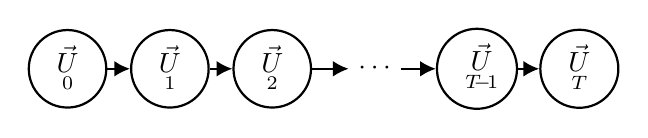
\begin{tikzpicture}[node distance=1.3cm, >={Latex[length=2mm, width=2mm]}, 
        obs/.style={circle, draw, align=center, text width = 3mm, minimum size=3mm, thick, font=\sffamily},
        lat/.style={rectangle, draw, align=center, text width = 6mm, minimum size=6mm, thick, font=\sffamily}]
        
        % Nodes
        \node[obs] (U0) {$\underset{0}{\vec{U}}$};
        \node[obs, right of=U0] (U1) {$\underset{1}{\vec{U}}$};
        \node[obs, right of=U1] (U2) {$\underset{2}{\vec{U}}$};
        \node[right of=U2] (dots) {$\cdots$};
        \node[obs, right of=dots] (UTb) {$\underset{T\!\!-\!1}{\vec{U}}$};
        \node[obs, right of=UTb] (UT) {$\underset{T}{\vec{U}}$};
        
        % Edges
        \draw[->, thick] (U0) -- (U1);
        \draw[->, thick] (U1) -- (U2);
        \draw[->, thick] (U2) -- (dots);
        \draw[->, thick] (dots) -- (UTb);
        \draw[->, thick] (UTb) -- (UT);
    \end{tikzpicture}
\end{center}
The full state of each $\vec{U}_i$ is generally unknown to us, so this joint prior distribution is not by itself of much value to us. To use the joint distribution as a posterior distribution, we need to introduce a likelihood to relate the state to some observations. For this, we describ the idea of the Information Operator (\cite{information_operator}) letting us impose constraints on the state-space representation of the function. For this, the idea of state-projection matrices is useful.
\definition{State Selection Matrices $E_i$}{
    It will be convenient to have an easy way of selecting a specific order derivative $q$ from the state $\vec{U}_i \in \reals^{n\cdot (1+q)}$. We can do so by projecting the full state onto the $q$-th derivative. 
    $$\begin{bmatrix} U \\ \frac{d}{d t} U \\ \cdots \\ \frac{d^q}{d t^q} U\end{bmatrix}$$ We can define the state-projection matrix $E_0$ for the $0$th derivative (the function) as 
    $$E_q = \begin{bmatrix}
        \textbf{I}_n & \textbf{0} & \cdots & \textbf{0}\\
        \textbf{0} & \textbf{0} & \cdots & \textbf{0}\\
        \vdots & \vdots & \ddots & \vdots \\
        \textbf{0} & \textbf{0} & \cdots & \textbf{0}\\
        \end{bmatrix}$$
}
\definition{Information Operator}{
    Although we might not know the complete state at each instant, there might
    We condition on partial observations of some of the time instances (the four blue dots in \ref{fig:iwps}). These optional partial observations can be expressed as $O_i \sim \mathcal{N}(h(\vec{U}_i), \sigma_h)$, where $h$ is a linear function of $\vec{U}_i$.
}
     Each $O_i$ is a function of only the state $\vec{U}_i$, and so the extended Bayesian Network including gaussian Ys takes the following form
    \begin{center}
        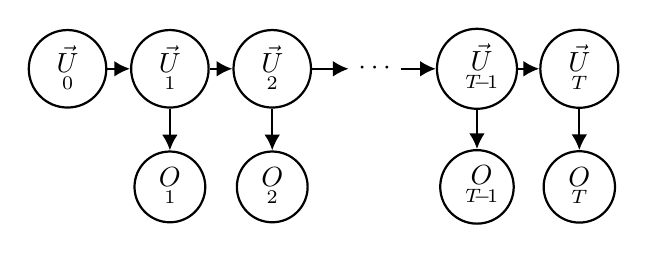
\begin{tikzpicture}[node distance=1.3cm, >={Latex[length=2mm, width=2mm]}, 
            obs/.style={circle, draw, align=center, text width = 3mm, minimum size=3mm, thick, font=\sffamily},
            lat/.style={rectangle, draw, align=center, text width = 6mm, minimum size=6mm, thick, font=\sffamily}]
            
            % Nodes
            \node[obs] (U0) {$\underset{0}{\vec{U}}$};
            \node[obs, right of=U0] (U1) {$\underset{1}{\vec{U}}$};
            \node[obs, right of=U1] (U2) {$\underset{2}{\vec{U}}$};
            \node[right of=U2] (dots) {$\cdots$};
            \node[obs, right of=dots] (UTb) {$\underset{T\!\!-\!1}{\vec{U}}$};
            \node[obs, right of=UTb] (UT) {$\underset{T}{\vec{U}}$};
            
            \node[obs, below of=U1, yshift=-0.2cm] (O1) {$\underset{1}{O}$};
        \node[obs, below of=U2, yshift=-0.2cm] (O2) {$\underset{2}{O}$};
        \node[obs, below of=UTb, yshift=-0.2cm] (OTb) {$\underset{T\!\!-\!1}{O}$};
        \node[obs, below of=UT, yshift=-0.2cm] (OT) {$\underset{T}{O}$};
        
        % Edges
        \draw[->, thick] (U0) -- (U1);
        \draw[->, thick] (U1) -- (U2);
        \draw[->, thick] (U2) -- (dots);
        \draw[->, thick] (dots) -- (UTb);
        \draw[->, thick] (UTb) -- (UT);
        
        \draw[->, thick] (U1) -- (O1);
        \draw[->, thick] (U2) -- (O2);
        \draw[->, thick] (UTb) -- (OTb);
        \draw[->, thick] (UT) -- (OT);    
    \end{tikzpicture}
\end{center}

How did we generate figures \ref{fig:iwps}? We express the factorized joint distribution of the Integrated Wiener Process using Matrix Fraction Decomposition for eqs. \ref{eq:easy_matrix_exponential} and \ref{eq:hard_matrix_exponential}, choose an initial distribution\footnote{The figures use a deterministic initial distribution $\vec{U}(0) \sim \mathcal{N}(\mathbf{0}^n, \mathbf{0}^{n \times n})$}.

The chain-structure of the bayesian network can be exploited to compute the posterior in time $O(|\mathbb{T}|n^3)$(\cite{probnum}) which increases linearly with time. The Kalman-filter and -smoother can be used to compute the full posterior distribution given linear (possibly noisy) transformations $Y_i$ of the state $\vec{U}_i$ at each time.
If one were to form the full joint distribution as one long mean-vector and covariance matrix, the cost of computing the posterior would be of order $O(|\mathbb{T}|^3n^3)$ by the cubic cost of matrix inversion required for the covariance matrix.




\subsection*{Hypothesis: Heat Prior, Wave Prior}
\definition{Heat Prior, Wave Prior}{What is it?}



\ifdefined\COMPILINGFROMMAIN
\else    
    \end{document}
\fi

\section{Information Operator}\label{sec:residual}
\input{../information_op/information_op.tex}

\section{Discretizing Prior}\label{sec:matrix_exponential}
\input{../matrix_exponential/matrix_exponential.tex}

\section{Kalman Filter}\label{sec:kalman_filter}
\input{../kalman_filter/kalman_filter.tex}

\section{Experiments}
\input{../experiments/experiments.tex}

\section{Results}
Use the \texttt{figure*} or \texttt{table*} environments for figures or tables spanning both columns.

\begin{figure*}[ht]
    \centering
    \includegraphics[width=0.8\textwidth]{../images/smiley.png}
    \caption{A wide figure spanning both columns.}
    \label{smileybotch}
\end{figure*}

\section{Conclusion}
Smiley er sej og er figur \ref{smileybotch}

\cite{example2024}
\printbibliography

\end{document}
